%%%  کلاس AUTthesis، نسخه آبان 1397
%%%   دانشگاه صنعتی امیرکبیر                 http://www.aut.ac.ir
%%%  تالار گفتگوی پارسی‌لاتک،       http://forum.parsilatex.com
%%%   آپدیت شده در آبان 95
%%%   پشتیبانی و راهنمایی          badali_farhad@yahoo.com
%%%
%%%   بازبینی و اصلاح شده در آبان ماه 1397
%%%  Tested via TeXstudio in TeXlive 2014-2018.
%%%

%-----------------------------------------------------------------------------------------------------
%        روش اجرا.: 2 بار F1 ، 2 بار  F11(به منظور تولید مراجع) ، دوبار Ctrl+Alt+I (به منظور تولید نمایه) و دو بار F1 -------> مشاهده Pdf
%%%%%%%%%%%%%%%%%%%%%%%%%%%%%%%%%%%%%%%%%%%%%%%%%%%%%%
%   TeXstudio as your IDE
%%  برای compile در TeXstudio تنها کافی است منوی Options->Configure TeXstudio را زده و در پنجره Configure TeXstudio در بخش Build گزینه Default Compiler را به XeLaTeX تغییر دهید. سند شما به راحتی compile خواهد شد.
%   F1 & F5 : Build & view
%   F6      : Compile
%   F7      : View
%   --------------
%%%%%%%%%%%%%%%%%%%%%%%%%%%%%%%%%%%%%%%%%%%%%%%%%%%%%%
%        اگر قصد نوشتن رساله دکتری را دارید، در خط زیر به جای msc،
%      کلمه phd را قرار دهید. کلیه تنظیمات لازم، به طور خودکار، اعمال می‌شود.
%%% !TEX TS-program = XeLaTeX
\documentclass[oneside,bsc,12pt]{AUTthesis}
%       فایل commands.tex را حتماً به دقت مطالعه کنید؛ چون دستورات مربوط به فراخوانی بسته زی‌پرشین 
%       و دیگر بسته‌ها و ... در این فایل قرار دارد و بهتر است که با نحوه استفاده از آنها آشنا شوید. توجه شود برای نسخه نهایی پایان‌نامه حتماً hyperref را 
%        غیرفعال کنید.


% در این فایل، دستورها و تنظیمات مورد نیاز، آورده شده است.
%-------------------------------------------------------------------------------------------------------------------
% در ورژن جدید زی‌پرشین برای تایپ متن‌های ریاضی، این سه بسته، حتماً باید فراخوانی شود.
\usepackage{amsthm,amssymb,amsmath,amsfonts}
% بسته‌ای برای تنطیم حاشیه‌های بالا، پایین، چپ و راست صفحه
\usepackage[top=30mm, bottom=30mm, left=25mm, right=30mm]{geometry}
% بسته‌‌ای برای ظاهر شدن شکل‌ها و تصاویر متن
\usepackage{graphicx}
\graphicspath{{figures/}}
\usepackage{color}
%بسته‌ای برای تنظیم فاصله عمودی خط‌های متن
\usepackage{setspace}
\usepackage{titletoc}
\usepackage{tocloft}
\usepackage{subcaption}
\usepackage{notoccite}
%با فعال کردن بسته زیر فوت‌نوت‌ها در هر صفحه ریست می‌شوند. حالت پیش‌فرض آن ریست شدن در هر فصل می‌باشد.
%\usepackage[perpage]{footmisc}
\usepackage{enumitem}
%\usepackage{titlesec}
% بسته‌ و دستوراتی برای ایجاد لینک‌های رنگی با امکان جهش
\usepackage[pagebackref=false,colorlinks,linkcolor=blue,citecolor=red]{hyperref}
\usepackage[nameinlink]{cleveref}%capitalize,,noabbrev
 \AtBeginDocument{%
    \crefname{equation}{برابری}{equations}%
    \crefname{chapter}{فصل}{chapters}%
    \crefname{section}{بخش}{sections}%
    \crefname{appendix}{پیوست}{appendices}%
    \crefname{enumi}{مورد}{items}%
    \crefname{footnote}{زیرنویس}{footnotes}%
    \crefname{figure}{شکل}{figures}%
    \crefname{table}{جدول}{tables}%
    \crefname{theorem}{قضیه}{theorems}%
    \crefname{lemma}{لم}{lemmas}%
    \crefname{corollary}{نتیجه}{corollaries}%
    \crefname{proposition}{گزاره}{propositions}%
    \crefname{definition}{تعریف}{definitions}%
    \crefname{result}{نتیجه}{results}%
    \crefname{example}{مثال}{examples}%
    \crefname{remark}{نکته}{remarks}%
    \crefname{note}{یادداشت}{notes}%
}
% چنانچه قصد پرینت گرفتن نوشته خود را دارید، خط بالا را غیرفعال و  از دستور زیر استفاده کنید چون در صورت استفاده از دستور زیر‌‌، 
% لینک‌ها به رنگ سیاه ظاهر خواهند شد که برای پرینت گرفتن، مناسب‌تر است
%\usepackage[pagebackref=false]{hyperref}
% بسته‌ لازم برای تنظیم سربرگ‌ها
\usepackage{fancyhdr}
% بسته‌ای برای ظاهر شدن «مراجع»  در فهرست مطالب
\usepackage[nottoc]{tocbibind}
% دستورات مربوط به ایجاد نمایه
\usepackage{makeidx,multicol}
\setlength{\columnsep}{1.5cm}

%%%%%%%%%%%%%%%%%%%%%%%%%%
\usepackage{verbatim}
\makeindex
\usepackage{sectsty}
% فراخوانی بسته زی‌پرشین و تعریف قلم فارسی و انگلیسی
\usepackage{xepersian}%[extrafootnotefeatures]
\SepMark{-}
%حتماً از تک لایو 2014 استفاده کنید.
\settextfont[Scale=1.2]{B Nazanin}
%\setlatintextfont{Times New Roman}
\renewcommand{\labelitemi}{$\bullet$}
%%%%%%%%%%%%%%%%%%%%%%%%%%
% چنانچه می‌خواهید اعداد در فرمول‌ها، انگلیسی باشد، خط زیر را غیرفعال کنید.
%در غیر اینصورت حتماً فونت PGaramond را نصب کنید.
%\setdigitfont[Scale=1.1]{PGaramond}%%Yas
%%%%%%%%%%%%%%%%%%%%%%%%%%
% تعریف قلم‌های فارسی اضافی برای استفاده در بعضی از قسمت‌های متن
\defpersianfont\nastaliq[Scale=2]{IranNastaliq}
\defpersianfont\chapternumber[Scale=3]{B Nazanin}
%\chapterfont{\centering}%
%%%%%%%%%%%%%%%%%%%%%%%%%%
% دستوری برای تغییر نام کلمه «اثبات» به «برهان»
\renewcommand\proofname{\textbf{برهان}}

% دستوری برای تغییر نام کلمه «کتاب‌نامه» به «منابع و مراجع«
\renewcommand{\bibname}{منابع و مراجع}


% Headings for every page of ToC, LoF and Lot
\setlength{\cftbeforetoctitleskip}{-1.2em}
\setlength{\cftbeforelottitleskip}{-1.2em}
\setlength{\cftbeforeloftitleskip}{-1.2em}
\setlength{\cftaftertoctitleskip}{-1em}
\setlength{\cftafterlottitleskip}{-1em}
\setlength{\cftafterloftitleskip}{-1em}
%%\makeatletter
%%%%\renewcommand{\l@chapter}{\@dottedtocline{1}{1em\bfseries}{1em}}
%%%%\renewcommand{\l@section}{\@dottedtocline{2}{2em}{2em}}
%%%%\renewcommand{\l@subsection}{\@dottedtocline{3}{3em}{3em}}
%%%%\renewcommand{\l@subsubsection}{\@dottedtocline{4}{4em}{4em}}
%%%%\makeatother


\newcommand\tocheading{\par عنوان\hfill صفحه \par}
\newcommand\lofheading{\hspace*{.5cm}\figurename\hfill صفحه \par}
\newcommand\lotheading{\hspace*{.5cm}\tablename\hfill صفحه \par}

\renewcommand{\cftchapleader}{\cftdotfill{\cftdotsep}}
\renewcommand{\cfttoctitlefont}{\hspace*{\fill}\LARGE\bfseries}%\Large
\renewcommand{\cftaftertoctitle}{\hspace*{\fill}}
\renewcommand{\cftlottitlefont}{\hspace*{\fill}\LARGE\bfseries}%\Large
\renewcommand{\cftafterlottitle}{\hspace*{\fill}}
\renewcommand{\cftloftitlefont}{\hspace*{\fill}\LARGE\bfseries}
\renewcommand{\cftafterloftitle}{\hspace*{\fill}}

%%%%%%%%%%%%%%%%%%%%%%%%%%
% تعریف و نحوه ظاهر شدن عنوان قضیه‌ها، تعریف‌ها، مثال‌ها و ...
%برای شماره گذاری سه تایی قضیه ها
\theoremstyle{definition}
\newtheorem{definition}{تعریف}[section]
\newtheorem{remark}[definition]{نکته}
\newtheorem{note}[definition]{یادداشت}
\newtheorem{example}[definition]{نمونه}
\newtheorem{question}[definition]{سوال}
\newtheorem{remember}[definition]{یاداوری}
\theoremstyle{theorem}
\newtheorem{theorem}[definition]{قضیه}
\newtheorem{lemma}[definition]{لم}
\newtheorem{proposition}[definition]{گزاره}
\newtheorem{corollary}[definition]{نتیجه}
%%%%%%%%%%%%%%%%%%%%%%%%
%%%%%%%%%%%%%%%%%%%
%%% برای شماره گذاری چهارتایی قضیه ها و ...
%%\newtheorem{definition1}[subsubsection]{تعریف}
%%\newtheorem{theorem1}[subsubsection]{قضیه}
%%\newtheorem{lemma1}[subsubsection]{لم}
%%\newtheorem{proposition1}[subsubsection]{گزاره}
%%\newtheorem{corollary1}[subsubsection]{نتیجه}
%%\newtheorem{remark1}[subsubsection]{نکته}
%%\newtheorem{example1}[subsubsection]{مثال}
%%\newtheorem{question1}[subsubsection]{سوال}

%%%%%%%%%%%%%%%%%%%%%%%%%%%%

% دستورهایی برای سفارشی کردن صفحات اول فصل‌ها
\makeatletter
\newcommand\mycustomraggedright{%
 \if@RTL\raggedleft%
 \else\raggedright%
 \fi}
\def\@makechapterhead#1{%
\thispagestyle{style1}
\vspace*{20\p@}%
{\parindent \z@ \mycustomraggedright
\ifnum \c@secnumdepth >\m@ne
\if@mainmatter

\bfseries{\Huge \@chapapp}\small\space {\chapternumber\thechapter}
\par\nobreak
\vskip 0\p@
\fi
\fi
\interlinepenalty\@M 
\Huge \bfseries #1\par\nobreak
\vskip 120\p@

}

%\thispagestyle{empty}
\newpage}
\bidi@patchcmd{\@makechapterhead}{\thechapter}{\tartibi{chapter}}{}{}
\bidi@patchcmd{\chaptermark}{\thechapter}{\tartibi{chapter}}{}{}
\makeatother

\pagestyle{fancy}
\renewcommand{\chaptermark}[1]{\markboth{\chaptername~\tartibi{chapter}: #1}{}}

\fancypagestyle{style1}{
\fancyhf{} 
\fancyfoot[c]{\thepage}
\fancyhead[R]{\leftmark}%
\renewcommand{\headrulewidth}{1.2pt}
}


\fancypagestyle{style2}{
\fancyhf{}
\fancyhead[R]{چکیده}
\fancyfoot[C]{\thepage{}}
\renewcommand{\headrulewidth}{1.2pt}
}

\fancypagestyle{style3}{%
  \fancyhf{}%
  \fancyhead[R]{فهرست نمادها}
  \fancyfoot[C]{\thepage}%
  \renewcommand{\headrulewidth}{1.2pt}%
}

\fancypagestyle{style4}{%
  \fancyhf{}%
  \fancyhead[R]{فهرست جداول}
  \fancyfoot[C]{\thepage}%
  \renewcommand{\headrulewidth}{1.2pt}%
}

\fancypagestyle{style5}{%
  \fancyhf{}%
  \fancyhead[R]{فهرست اشکال}
  \fancyfoot[C]{\thepage}%
  \renewcommand{\headrulewidth}{1.2pt}%
}

\fancypagestyle{style6}{%
  \fancyhf{}%
  \fancyhead[R]{فهرست مطالب}
  \fancyfoot[C]{\thepage}%
  \renewcommand{\headrulewidth}{1.2pt}%
}

\fancypagestyle{style7}{%
  \fancyhf{}%
  \fancyhead[R]{نمایه}
  \fancyfoot[C]{\thepage}%
  \renewcommand{\headrulewidth}{1.2pt}%
}

\fancypagestyle{style8}{%
  \fancyhf{}%
  \fancyhead[R]{منابع و مراجع}
  \fancyfoot[C]{\thepage}%
  \renewcommand{\headrulewidth}{1.2pt}%
}
\fancypagestyle{style9}{%
  \fancyhf{}%
  \fancyhead[R]{واژه‌نامه‌ی فارسی به انگلیسی}
  \fancyfoot[C]{\thepage}%
  \renewcommand{\headrulewidth}{1.2pt}%
}
%


%دستور حذف نام لیست تصاویر و لیست جداول از فهرست مطالب
\newcommand*{\BeginNoToc}{%
  \addtocontents{toc}{%
    \edef\protect\SavedTocDepth{\protect\the\protect\value{tocdepth}}%
  }%
  \addtocontents{toc}{%
    \protect\setcounter{tocdepth}{-10}%
  }%
}
\newcommand*{\EndNoToc}{%
  \addtocontents{toc}{%
    \protect\setcounter{tocdepth}{\protect\SavedTocDepth}%
  }%
}
\newcounter{savepage}
\renewcommand{\listfigurename}{فهرست اشکال}
\renewcommand{\listtablename}{فهرست جداول}
%\renewcommand\cftsecleader{\cftdotfill{\cftdotsep}}
%%%%%%%%%%%%%%%%%%%%%%%%%%%%%
%%%%%%%%%%%%%%%%%%%%%%%%%%%%
\begin{document}
\baselineskip=.75cm
\linespread{1.75}
%% -!TEX root = AUTthesis.tex
% در این فایل، عنوان پایان‌نامه، مشخصات خود، متن تقدیمی‌، ستایش، سپاس‌گزاری و چکیده پایان‌نامه را به فارسی، وارد کنید.
% توجه داشته باشید که جدول حاوی مشخصات پروژه/پایان‌نامه/رساله و همچنین، مشخصات داخل آن، به طور خودکار، درج می‌شود.
%%%%%%%%%%%%%%%%%%%%%%%%%%%%%%%%%%%%
% دانشکده، آموزشکده و یا پژوهشکده  خود را وارد کنید
\faculty{دانشکده مهندسی کامپیوتر}
% گرایش و گروه آموزشی خود را وارد کنید
\department{گرایش معماری سیستم‌های کامپیوتری}
% عنوان پایان‌نامه را وارد کنید
\fatitle{پياده‌سازی سيستم لرزه‌نگار جهت نگهداری و تعميرات پيش‌بينانه تجهيزات بر بستر اينترنت اشياء}
% نام استاد(ان) راهنما را وارد کنید
\firstsupervisor{دکتر حمیدرضا زرندی}
%\secondsupervisor{استاد راهنمای دوم}
% نام استاد(دان) مشاور را وارد کنید. چنانچه استاد مشاور ندارید، دستور پایین را غیرفعال کنید.
%\firstadvisor{نام کامل استاد مشاور}
%\secondadvisor{استاد مشاور دوم}
% نام نویسنده را وارد کنید
\name{میلاد}
% نام خانوادگی نویسنده را وارد کنید
\surname{اسرافیلیان نجف‌آبادی}
%%%%%%%%%%%%%%%%%%%%%%%%%%%%%%%%%%
\thesisdate{تیر ۱۴۰۲}

% چکیده پایان‌نامه را وارد کنید
\fa-abstract{در سال‌های اخیر اینترنت اشیاء به یکی از داغ‌ترین موضوعات فناوری تبدیل شده‌است. کاربرد این فناوری در تمامی حوزه‌های زندگی انسان و همچنین پیشرفت‌های اخیر در حوزه‌های جمع‌آوری داده، شبکه و هوش مصنوعی باعث شده‌اند که اینترنت اشیاء مورد توجه محققان قرار گیرد. یکی از چالش‌های موجود در صنایع و کارخانه‌ها تعویض بهینه قطعات است. با توجه به نبود اطلاعات کافی برای تحلیل وضعیت قطعات، راه‌حل مناسب برای اطمینان از کارکرد خط تولید، استفاده از متخصصان جهت بازرسی از وضعیت تجهیزات یا تعویض آنها بدون توجه به وضعیت فعلی و صرفا طبق زمان‌بندی قبلی است. این راه‌حل‌ها علاوه بر نداشتن دقت لازم، هزینه و زمان زیادی بر صنایع تحمیل می‌کنند. در این پروژه قصد داریم که با استفاده از ترکیب اینترنت اشیاء و هوش مصنوعی، چارچوبی برای تحلیل داده‌های لرزش تجهیزات ارائه گردد تا با استفاده از آن بتوان عمر مفید باقیمانده قطعات را بخوبی پیش‌بینی کرد. همچنین با استفاده از درگاه مبتنی بر وب، نتایج حاصله به افراد متخصص نشان داده شود تا بتوانند برنامه‌ریزی دقیقی برای نگهداری و تعمیر تجهیزات ارائه کنند. با بکارگیری این رویکرد هزینه و وقت صرف‌شده برای تعویض قطعات به‌شکل چشمگیری کاهش می‌یابد.}


% کلمات کلیدی پایان‌نامه را وارد کنید
\keywords{اینترنت اشیاء، نگهداری پیش‌بینانه، اینترنت اشیاء صنعتی، نگهداری سیستم سایبری-فیزیکی}



\AUTtitle
%%%%%%%%%%%%%%%%%%%%%%%%%%%%%%%%%%
\vspace*{7cm}
\thispagestyle{empty}
\begin{center}

\includegraphics[height=5cm,width=12cm]{besm}
\end{center}
% تاییدیه دفاع
\newpage
\thispagestyle{empty}
%\fontsize{18pt}{19pt}\selectfont

\section*{صفحه فرم ارزیابی و تصویب پایان نامه- فرم تأیید اعضاء كميته دفاع}

\fontsize{12pt}{14pt}\selectfont
%\renewcommand{\baselinestretch}{1.5}
\vspace*{1cm}
   در این صفحه فرم دفاع یا تایید و تصویب پایان نامه موسوم به فرم کمیته دفاع- موجود در پرونده آموزشی- را قرار دهید.
\vspace*{1cm}


\subsection*{نکات مهم:}
 
\begin{itemize}
\item
	نگارش پایان نامه/رساله باید به
	{\color{red}
		زبان فارسی
	}
	و بر اساس آخرین نسخه دستورالعمل و راهنمای تدوین پایان نامه های دانشگاه صنعتی امیرکبیر باشد.(دستورالعمل و راهنمای حاضر)
\item رنگ جلد پایان نامه/رساله چاپي كارشناسي، كارشناسي ارشد و دكترا  بايد به ترتيب مشكي، طوسي و سفيد رنگ باشد.  
\item چاپ و صحافی پایان نامه/رساله بصورت
{\color{red}
	پشت و رو(دورو)
}
بلامانع است و انجام آن توصيه مي شود. 
\end{itemize}
%%%%%%%%%%%%%%%%%%%%%%%%%%%%%%%%%%%%%%%%%%%%%%%%%%%%%%%%%%%%%%%%%%%%%%%%%%%%%%%%%%%%%%%%%%%%%%%%%%
%%%%%%%%%%%%%%%%%%%%%%%%%%%%%%%%%%%%%%%%%%%%%%%%%%%%%%%%%%%%%%%%%%%%%%%%%%%%%%%%%%%%%%%%%%%%%%%%%%
\newpage
\thispagestyle{empty}
\begin{picture}(50,50)
  \put(17,0){
\includegraphics[scale=1.1]{fa-logo}}
  \put(4.5,-13){\footnotesize{دانشگاه صنعتی امیرکبیر}}
  \put(10.5,-27){\footnotesize{(پلی‌تکنیک تهران)}}
  \put(170,30){\bf{به نام خدا}}
  \put(140,-5){\Large\bf{تعهدنامه اصالت اثر}}
  \put(310,0){تاریخ: \datethesis}
\end{picture}

\vspace*{2.5cm}

اينجانب {\bf{\fname\lname}} متعهد می‌شوم که مطالب مندرج در این پایان‌نامه حاصل کار پژوهشی اینجانب تحت نظارت و راهنمایی اساتید دانشگاه صنعتی امیرکبیر بوده و به دستاوردهای دیگران که در این پژوهش از آنها استفاده شده است مطابق مقررات و روال متعارف ارجاع و در فهرست منابع و مآخذ ذکر گردیده است. این پایان‌نامه قبلاً برای احراز هیچ مدرک هم‌سطح یا بالاتر ارائه نگردیده است.

در صورت اثبات تخلف در هر زمان، مدرک تحصیلی صادر شده توسط دانشگاه از درجه اعتبار ساقط بوده و دانشگاه حق پیگیری قانونی خواهد داشت.


کلیه نتایج و حقوق حاصل از این پایان‌نامه متعلق به دانشگاه صنعتی امیرکبیر می‌باشد. هرگونه استفاده از نتایج علمی و عملی، واگذاری اطلاعات به دیگران یا چاپ و تکثیر، نسخه‌برداری، ترجمه و اقتباس از این پایان نامه بدون موافقت کتبی دانشگاه صنعتی امیرکبیر ممنوع است. 
نقل مطالب با ذکر مآخذ بلامانع است.\\
\vspace{2.5cm}


{\centerline {\bf{\fname\lname}}}
\vspace*{.2cm}
{\centerline{امضا}}
%%%%%%%%%%%%%%%%%%%%%%%%%%%%%%%%%
% چنانچه مایل به چاپ صفحات «تقدیم»، «نیایش» و «سپاس‌گزاری» در خروجی نیستید، خط‌های زیر را با گذاشتن ٪  در ابتدای آنها غیرفعال کنید.
% پایان‌نامه خود را تقدیم کنید
% نیایش خود را در فایل زیر بنویسید.
\begin{acknowledgementpage}

\vspace{1.5cm}

{\nastaliq
{
تقدیم به

آنکه جز به فضلش امیدی نیست...
}}\end{acknowledgementpage}
\newpage
% سپاسگزاری را در فایل زیر بنویسید.
%%%%%%%%%%%%%%%%%%%%%%%%%%%%%%%%%%%%
\newpage\thispagestyle{empty}
% سپاس‌گزاری
{\nastaliq
سپاس‌گزاری
}
\\[2cm]

‫ﺍﺯ‬‫ﭘﺪﺭ‬ ‫ﻭ‬ ‫ﻣﺎﺩﺭﻡ‬ ‫ﻛﻪ‬ ‫ﻫﻤﻮﺍﺭﻩ‬ ‫ﺩﺭ‬ ‫ﻣﻮﺍﺟﻬﻪ‬ ‫ﺑﺎ‬ ‫ﺳﺨﺘﻲ‬‌‫ﻫﺎی ‬‫ﺍﻳﻦ‬ ‫ﺩﻧﻴﺎ‬ ‫ﺩﻟﺴﻮﺯﺍﻧﻪ‬ ‫ﻫﻤﺮﺍﻫﻢ‬ ‫ﺑﻮﺩﻩ‬‌‫ﺍﻧﺪ؛‬

‫ﺍﺯ‬‫ﺍﺳﺘﺎﺩ‬ ‫ﺑﺰﺭﮔﻮﺍﺭﻡ‬ ‫ﺟﻨﺎﺏ‬ ‫ﺁﻗﺎی‬ ‫ﺩﻛﺘﺮ‬ ‫حمیدرضا زرندی ‫ﻛﻪ‬ ‫ﺑﺎ‬ ‫ﺣﺴﻦ‬ ‫ﺧﻠﻖ‬ ‫ﻭ‬ ‫ﮔﺸﺎﺩﻩ‬‌‫ﺭﻭیی‪ ،‬‬‫ﺭﻫﻨﻤﻮﺩﻫﺎی‬
‫ﺷﺒﺎﻧﻪ‬‫ﺭﻭﺯی ‬‫ﺧﻮﺩ‬ ‫ﺭﺍ‬ ‫ﺍﺯ‬ ‫ﻣﻦ‬ ‫ﺩﺭﻳﻎ‬ ‫ﻧﻜﺮﺩﻩ‬‌‫ﺍﻧﺪ؛‬

‫ﻭ ‬‫ﺍﺯ‬ ‫ﺳﺎﻳﺮ‬ ‫ﻋﺰﻳﺰﺍنی‬ ‫ﻛﻪ‬ ‫ﺩﺭ‬ ‫ﻛﻨﺎﺭﺷﺎﻥ‬ ‫ﺍﻳﻦ‬ ‫نتیجه‬ ‫ﺣﺎﺻﻞ‬ ‫ﺁﻣﺪ‬ ‫ﻛﻤﺎﻝ‬ ‫ﺗﺸﻜﺮ‬ ‫ﻭ‬ ‫ﻗﺪﺭﺩﺍنی ‫ﺭﺍ‬ ‫ﺩﺍﺭﻡ‪.‬‬












% با استفاده از دستور زیر، امضای شما، به طور خودکار، درج می‌شود.
\signature








%%%%%%%%%%%%%%%%%%%%%%%%%%%%%%%%%%%%%%%%%
%%%%%%%%%%%%%%%%%%%%%%%%%%%%%%%%%کدهای زیر را تغییر ندهید.
\newpage\clearpage

\pagestyle{style2}

\vspace*{-1cm}
\section*{\centering چکیده}
%\addcontentsline{toc}{chapter}{چکیده}
\vspace*{.5cm}
\ffa-abstract
\vspace*{2cm}


{\noindent\large\textbf{واژه‌های کلیدی:}}\par
\vspace*{.5cm}
\fkeywords
% دستور زیر برای شماره گذاری صفحات قبل از فصل اول با حروف ابجد است.
\pagenumbering{alph}
%-----------------------------------------------------------------------------
% فایل زیر دستورات مربوط به نمایش صفحات فهرست مطالب- فهرست اشکال و جداول است.
%{\pagestyle{style2}
%\tableofcontents}\newpage
%
%\listoffigures
\cleardoublepage
\pagestyle{style6}
\tableofcontents
\pagestyle{style6}
\cleardoublepage
%اگر لیست تصاویر و لیست جداول ندارید ، کدهای زیر را با گذاشتن % در ابتدای آنها، غیرفعال کنید.
\BeginNoToc
%============
\addtocontents{lof}{\lofheading}% add heading to the first page in LoF
\pagestyle{style5}
\listoffigures
\thispagestyle{style5}
\cleardoublepage
%============
\addtocontents{lot}{\lotheading}% add heading to the first page in LoT
\thispagestyle{style4}
\listoftables
\thispagestyle{style4}
%============
%\cleardoublepage
%
\cleardoublepage
\setcounter{savepage}{\arabic{page}}
\mainmatter
\addtocontents{toc}{\tocheading}% add heading to the first page in ToC, after frontmatter entries
\EndNoToc
% در صورت تمایل می‌توانید با فعال کردن دستور بالا، لیست تصاویر را به  پایان‌نامه خود اضافه کنید.
%-------------------------------------------------------------------------symbols(فهرست نمادها)
% وجود لیست نمادها الزامیست.(لطفاً نمادهای خود را جایگذین نمادهای پیش‌فرض کنید.)
%%%%%%%%%%%%%

{\centering\LARGE\textbf{فهرست نمادها}\par}%

\pagenumbering{alph}
\setcounter{page}{\thesavepage}
%\setcounter{page}{6}
\vspace*{1cm}

\pagestyle{style3}
%\thispagestyle{empty}
%\addcontentsline{toc}{chapter}{فهرست نمادها}
\symb{\text{ نماد}}{مفهوم}
\\
%مقادیر بالا را تغییر ندهید
%%%%%%%%%%%%%%%%%%%%%%%%%%%%%%%%%%%%%%%%%%%%%%%%%%%%%%%%%
\symb{K}{
تعداد همه‌ی نمونه‌های موجود در یک اندازه‌گیری
}
\symb{n}{
گره $n$ ام
}
\symb{m}{
اندازه‌گیری $m$ ام
}
\symb{k}{
نمونه‌ی $k$ ام در یک اندازه‌گیری
}
\symb{a_{nmk}}{
بردار سه‌بعدی مربوط به اندازی‌گیری لرزش
}
\symb{\hat{a}}{
بردار هنجار‌شده $a$
}
\symb{g}{
شتاب گرانش زمین
}
%%%%%%%%%%%%%%%%%%%%%%%%%%%%%%%%%%%%%%%

\thispagestyle{style3}
\newpage
%\pagestyle{style1}
%%%%%%%%%%%%%%%%%%%%%%%%%%%%%%%%%%%%


\pagenumbering{arabic}
\pagestyle{style1}
%--------------------------------------------------------------------------chapters(فصل ها)
\chapter{مقدمه}

\section{تعمیر و نگهداری}

در دنیای نوین امروز، وابستگی به فناوری و صنایع مختلف برای ارائه خدمات و تولید محصولات مورد نیاز بشدت افزایش یافته‌است. در نتیجه این افزایش، تعداد کارخانه‌ها و تجهیزات برای رفع این نیازها نیز افزایش یافته‌است. همه تجهیزات و وسایل پس از استفاده زیاد دچار نقص و فراوانی می‌شوند. خرابی تجهیزات در کارخانه‌ها و حطوط تولید پدیده‌ای نامطلوب است. خرابی تجهیزات باعث ایست خط تولید و وارد کردن ضرر مالی به صاحبان کارخانه‌ها خواهد شد. به‌همین دلیل، تعمیر و نگهداری تجهیزات اهمیت بالایی دارد. 

سیاست‌های انجام تعمیرات و نگهداری به سه دسته اصلی تقسیم می‌شوند؛ که در \cref{MS} \cite{zhao2022review} آورده شده‌است:

\begin{figure}[!h]
\centering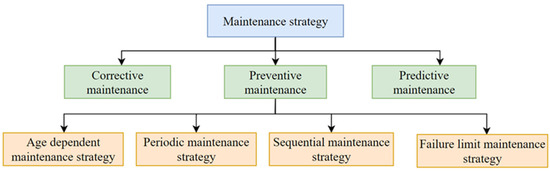
\includegraphics[scale=1]{maintenance_strategy.png}
\caption{سیاست‌های انجام تعمیرات و نگهداری}\label{MS}
\end{figure}

این سیاست‌ها عبارتند از:
\begin{itemize}
\item نگهداری اصلاحی\LTRfootnote{Corrective Maintenance}: این نوع نگهداری با اتفاق افتادن خرابی رخ می‌دهد و تنها در صورت خرابی قطعه تعمیر انجام می‌شود. همانطور که مشخص است در این حالت روند کارکرد عادی متوقف می‌شود: به‌علاوه، در این حالت تعمیر می‌تواند با تاخیر انجام شود زیرا ممکن است در لحظه قطعات مورد نیاز برای تعمیر موجود نباشد. از این سیاست بیشتر به‌عنوان مکملی برای سیاست‌های بعدی استفاده می‌شود\cite{zhao2022review}.

\item نگهداری پیش‌گیرانه\LTRfootnote{Preventive Maintenance}: در این حالت، نگهداری و تعمیر بر اساس رابطه بین نرخ خرابی، توزیع زمان خرابی و سایر آستانه‌هایی که از تعداد زیادی از آمارهای خرابی بدست می‌آید زمان‌بندی می‌شود. در واقع در این نوع نگهداری هدف کاهش احتمال خرابی قطعات است. این نوع نگهداری با توجه به نوع اطلاعات به سیاست‌های وابسته عمر،\LTRfootnote{Age Dependent Strategies} سیاست‌های دوره‌ای\LTRfootnote{Periodic Strategies}، سیاست‌های ترتیبی\LTRfootnote{Sequential Strategies} و سیاست‌های محدودکننده خرابی\LTRfootnote{Failure Limited Strategies} تقسیم می‌شوند\cite{zhao2022review}.

\item نگهداری پیش‌بینانه\LTRfootnote{Predictive Maintenance}: این نوع نگهداری بر روند کاهش کارایی قطعات با استفاده از وضعیت آنها نظارت کرده، وضعیت آنها را در آینده پیش‌بینی می‌کند و مداوم برنامه تعمیر و نگهداری را بروزرسانی می‌کند، تا اینکه شرایط توقف بروزرسانی برآورده شود. با توجه به این ویژگی، این سیاست فقط برای تجهیزاتی که وضعیت آنها قابل نظارت است می‌تواند استفاده شود\cite{zhao2022review}.
\end{itemize} 

\section{راهکار پیشنهادی}

با توجه به اهمیت نگهداری و نقش نگهداری اصولی در کاهش هزینه، در این پروژه به ایجاد چارچوبی مناسب برای ارائه راهکاری بر مبنای سیاست نگهداری پیش‌بینانه می‌پردازیم. یکی از نیازهای این سیاست حجم زیادی از داده جمع‌آوری شده از وضعیت تجهیزات برای پیش‌بینی دقیق است. در این پروژه در بستر اینترنت اشیاء\LTRfootnote{Internet of Things} داده‌های لرزش با استفاده از سنسور \lr{MEMS}\LTRfootnote{Micro Electric Mechanical Sensor} جمع‌آوری شده و در زمان‌های مشخص با استفاده از پروتکل زیگبی\LTRfootnote{Zigbee Protocol} برای دروازه\LTRfootnote{Gateway} فرستاده می‌شود. پس از جمع‌آوری حجم مشخصی از داده‌هااطلاعات برای پردازش بیشتر به سرور فرستاده می‌شوند. در انتها نیز اطلاعات پردازش‌شده و تخمین عمر مفید باقیمانده\LTRfootnote{Remaining Useful Lifetime(RUL)} در یک صفحه وب نمایش داده می‌شود.

\section{کارهای مشابه}
در \cite{tinga2010application} مدلی برای خرابی قطعات مبتنی بر میزان استفاده از تجهیزات و بار داخلی آنها ارائه شده‌است اما مدل ارائه‌شده محدود به یک مدل تجهیزات است و برای استفاده در سایر مدل‌ها نظارت مجدد لازم است. در \cite{wu2007neural} رویکردی مبتنی بر شبکه عصبی جهت پیش‌بینی عمر مفید باقیمانده تجهیزات چرخشی ارائه شده‌است اما تنها مختص به این دسته از تجهیزات است. در \cite{kaiser2009predictive} رویکردی مبتنی بر شبکه عصبی جهت پیش‌بینی زمان نگهداری و تعمیرات تجهیزات بر اساس مدل خرابی و کارایی آنها ارائه می‌شود اما در یک محیط شبیه‌سازی‌شده و کنترل‌شده آزمایش شده‌است و در هنگام استفاده در محیط واقعی غیرعملی است.

بطور کلی در پژوهش‌های یادشده رویکرد‌های ارائه‌شده مختص نوع خاصی از تجهیزات است و در یک مجیط آزمایشگاهی و کنترل‌شده ارزیابی شده‌اند. در حالیکه در این پروژه با استفاده از داده‌های جمع‌آوری‌شده از قطعات مختلف سعی کرده‌ایم رویکردی کلی و مناسب محیط واقعی و صنعتی ارائه دهیم.

\chapter{طریقه‌ی مرجع نویسی و واژه‌نامه‌}
\section{طریقه‌ی مرجع نویسی}
برای نوشتن مراجع پایان نامه، برای راحتی کار به صورت زیر عمل می‌کنیم:
\subsection{بارگیری مراجع}
در ابتدا مراجع را باید از سایت‌های معتبر بارگیری کنیم، مثلا برای ارجاع دادن به مقاله‌ی
\lr{A classification of some Finsler connections and their applications}
ابتدا به سایت
\href{scholar.google.com}{گوگل اسکولار} 
رفته و این مقاله را جستجو می‌کنیم. پس از پیدا کردن این مقاله، مانند شکل زیر، در زیر نام و چکیده‌ی مقاله، $5$ گزینه وجود دارد که عبارتند از:\\

\begin{enumerate}
\item \lr{ Cited by}

\item \lr{ Related articles}

\item \lr{ All 6 versions}

\item \lr{ Cite}

\item \lr{ Save}
\end{enumerate}
\begin{figure}[!h]
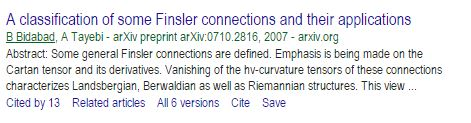
\includegraphics[height=3cm]{bidabad}
\caption{نمونه یک مقاله در گوگل اسکولار}
\end{figure}
در اینجا ما به گزینه‌ی چهارم یعنی
\lr{ Cite}
احتیاج داریم. بر روی آن کلیک کرده و پنجره‌ای مانند
\cref{fig.2}
باز می‌شود که دارای $4$ گزینه‌ی زیر است:
\begin{enumerate}
\item \lr{BibTeX}

\item \lr{EndNote}

\item \lr{RefMan}

\item \lr{RefWorks}
\end{enumerate}
\begin{figure}
\centering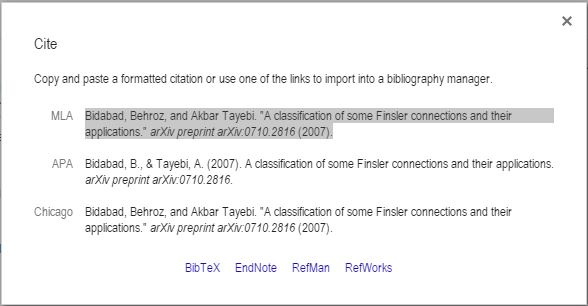
\includegraphics[scale=.6]{bibref}
\caption{پنجره‌ی باز شده در گوگل اسکولار}\label{fig.2}
\end{figure}
روی گزینه‌ی اول، یعنی
\verb;BibTeX;
کلیک کرده و همه‌ی نوشته‌های پنجره‌ی باز شده را مانند زیر، کپی کرده و در فایل
\verb;references.bib;
موجود در فایل
\verb;AUTthesis;
پیست می‌کنیم. سپس کلیدهای
\verb;Ctrl+s;
را می‌زنیم تا فایل ذخیره شود.\\
\begin{latin}
	\normalsize
\begin{verbatim}
@ article{bidabad2007classification,
title={A classification of some Finsler connections and their applications},
author={Bidabad, Behroz and Tayebi, Akbar},
journal={arXiv preprint arXiv:0710.2816},
year={2007}
}
\end{verbatim}
\end{latin}
\subsection{روش ارجاع در متن}
برای ارجاع دادن به مقاله‌ی بالا، باید در جایی که می‌خواهید ارجاع دهید، دستور زیر را تایپ کنید:
\begin{latin}
\lr{$\backslash$cite\{bidabad2007classification\}}
\end{latin}
همانطور که مشاهده می‌کنید از کلمه‌ای که در سطر اول ادرس مقاله آمده (یعنی کلمه‌ی پس از
\lr{@article$\lbrace$})
استفاده کرده‌ایم. پس از دستور فوق، به صورت \cite{bidabad2007classification} و \cite{aa} مرجع خواهد خورد. توجه شود که در صورتی مراجع چاپ خواهند شد که در متن به انها ارجاع داده شده باشد. همچنین برای ارجاع چندتایی از دستور 
\lr{$\backslash$cite\{name1, name2,...\}}
استفاده کنید که به‌صورت \cite{najafi2008finsler, zakeri, najafi} ارجاع خواهند خورد.
\subsection{روش اجرای برنامه}
ابتدا فایل
\verb;AUT_thesis.tex;
را باز کرده و آن را دو بار اجرا کنید. سپس حالت اجرا را از 
\verb;Build Quick;
به حالت
\verb;Bibtex;
تغییر داده و دوباره برنامه را اجرا کنید. دو بار دیگر برنامه را در حالت 
\verb;Build Quick;
اجرا کرده و نتیجه را مشاهده کنید. در این روش تمامی مراجع بر اساس اینکه کدام یک در متن زودتر به آن ارجع داده شده لیست خواهند شد.
\subsection{مراجع فارسی}
برای نوشتن مراجع فارسی باید به صورت دستی، در همان فایل قبلی به صورت زیر عمل می‌کنیم:
\begin{LTR}
\noindent\verb;@article{manifold,;\\
\verb;title={;منیفلد هندسه\verb;},;\\
\verb;author={;بیدآباد دکتربهروز \verb;},;\\
\verb;journal{; امیرکبیر صنعتی دانشگاه\verb;},;\\
\verb;year={1389},;\\
\verb;LANGUAGE={Persian};\\
\verb;};
\end{LTR}
همانطور که مشاهده می‌کنید تنها تفاوت آن با حالت مراجع انگلیسی، سطر آخر آن می‌باشد که زبان را مشخص می‌کند که حتماً باید نوشته شود.
\section{راهنمای واژه‌نامه}

به دلیل پیچیدگی واژه‌نامه‌های موجود در سایت پارسی لاتک، از روش زیر برای نوشتن واژه‌نامه استفاده کنید:

ابتدا با استفاده از اکسل، واژه های خود را یک‌بار براساس حروف الفبای فرسی و بار دیگر انگلیسی مرتب کنید. سپس واژه ها را در فایل \lr{dicen2fa} و \lr{dicfa2en} قرار دهید.

\section{ساخت نمایه}\label{Namaye}
\subsection{ساخت نمایه}
 \begin{enumerate}

\item
کلمات مورد نظر خود مثلا \lr{word} با دستور \verb|\index{word}| ایندکس کنید.
\item
نحوه‌ی اجرای \lr{Make Index}   در ویرایشگرهای \lr{TeX Maker} و \lr{TeX Works}:
\begin{itemize}
\item  تک‌میکر: از منوی \lr{Tools} گزینه‌ی \lr{Xindy Make Index} را کلیک کنید یا از دکمه‌‌های میانبر \lr{Ctrl+Alt+I} استفاده کنید.

\item  تک‌ورکز: ابتدا باید مثل عکس زیر تنظیم  و سپس گزینه‌ی \lr{Xindy Make Index}  انتخاب و روی دکمه‌ی سبز رنگ کلیک کنید یا از دکمه‌های  \lr{Ctrl+T} استفاده کنید.

\begin{figure}[!h]
\centerline{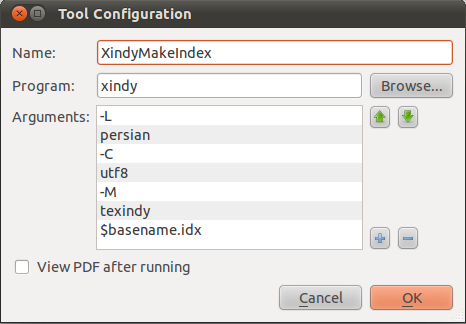
\includegraphics[width=.5\textwidth]{Xindy_Make_Index.png}}
\caption{تنظیمات مربوط به تک‌ورکز}
\end{figure}

\end{itemize}
 \end{enumerate}
 
 \index{کتاب}
\index{پارسی‌لاتک}
\index{بی‌دی}
\index{سوال}
\index{عنصر}
\index{گزینه}
\index{ژاکت}
\index{مرکز دانلود}
\index{اجرا}
\index{تک‌لایو}
\index{ثالث}
\index{جهان}
\index{چهار}
\index{حمایت}
\index{خواهش}
\index{دنیا}
\index{زی‌پرشین}
\index{ریحان}
\index{شیرین}
\index{صمیمی}
\index{ضمیر}
\index{طبیب}
\chapter{پیاده‌سازی سیستم}

در این قسمت نحوه‌ی اجرای پروژه را بطور کامل توضیح خواهیم داد. در هر قسمت ساختار فایل‌ها، نحوه‌ی پیاده‌سازی و چالش‌هایی که با آن مواجه بودیم به‌همراه نحوه‌ی حل آنها را توضیح خواهیم داد.

\section{معماری کلی سیستم}

برای درک بهتر این پروژه، نمایی کلی از سیستم و نحوه عملکرد آن را همانطور که در \cref{fig:system_overview} نشان داده شده است، ارائه خواهیم داد. این پروژه در چندین محل صنعتی مستقر خواهد شد. در هر کارخانه چندین میکروکنترلر آردوینو، با یک سنسور لرزش و یک فرستنده گیرنده زیگبی متصل، روی هر قطعه از تجهیزات نصب شده است. داده‌ها در زمان‌های برنامه‌ریزی‌شده حس می‌شوند و سپس به دروازه‌ای در کارخانه ارسال می‌شوند. دروازه اطلاعاتی را که از فرستنده‌گیرنده‌های زیگبی می‌آید را جمع‌آوری می‌کند تا زمانی که به یک آستانه‌ی از پیش تعریف‌شده برسد. سپس دروازه با سرور مرکزی احراز هویت می‌شود و سپس داده‌های جمع‌آوری‌شده را با پروتکل \lr{HTTP} به سرور ارسال می‌کند. در سرور مراحل پیش‌پردازش لازم انجام می‌شود و سپس داده‌ها در پایگاه داده‌ی سری زمانی ذخیره می‌شوند. سپس مدل یادگیری ماشین با داده‌های قبلی و جدید اجرا می‌شود تا پیش‌بینی دقیق‌تری درباره طول عمر مفید باقیمانده تجهیزات به ما ارائه دهد. در صورت درخواست، تمام داده‌های تحلیلی و پیشبینی‌ها از طریق داشبورد مدیریت قابل‌دسترسی است. متخصصان می‌توانند از این داده‌ها برای برنامه‌ریزی زمان نگهداری مناسب استفاده کنند.

\begin{figure}[!h]
\centering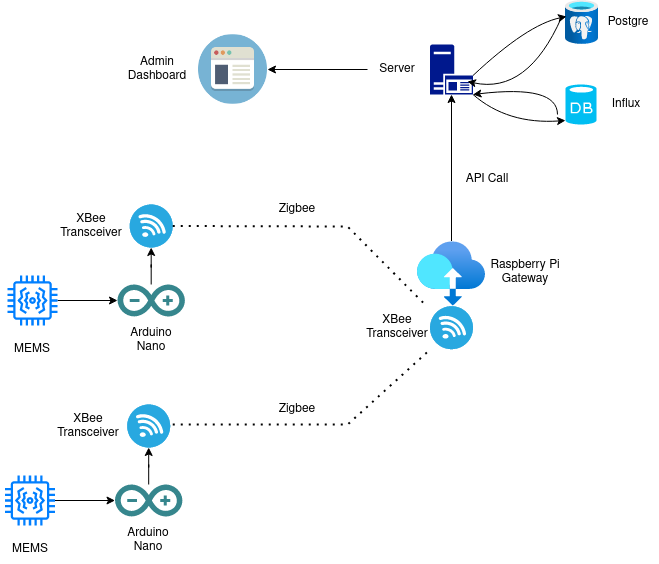
\includegraphics[scale=.6]{system_overview.png}
\caption{نمای کلی سیستم}\label{fig:system_overview}
\end{figure}

\section{گره انتهایی و آردوینو}

برای پیاده‌سازی گره انتهایی، سه بخش را باید پیاده‌سازی میکردیم که عبارتند از:

\begin{itemize}
\item خواندن از حسگر و نمونه‌برداری
\item تشکیل فریم زیگبی و نوشتن در درگاه سریال
\item خوابیدن و بیدارشدن در بازه‌های زمانی مشخص
\end{itemize}

در ادامه هر بخش را توضیح می‌دهیم.

\subsection{خواندن از حسگر و نمونه‌برداری}

حسگر \lr{ADXL345} چندین پارامتر دارد که باید در زمان راه‌اندازی تنظیم شوند. برای انجام پیکربندی و همچنین خواندن داده‌های حسگرها بدون نیاز به استفاده مستقیم از پروتکل \lr{I2C}، از کتابخانه\LTRfootnote{Adafruit\_ADXL345\_U.h} استفاده کرده‌ایم. یکی از پارامترها محدوده شتاب است که با تابع \lr{setRange} تنظیم می‌شود. محدوده مجاز ۲، ۴، ۸ یا ۱۶ برابر شتاب گرانش زمین است. اما هرچه دامنه بزرگتر شود، داده‌ها دقت کمتری پیدا می‌کنند. از آنجایی که یک قطعه از تجهیزات حتی زمانی که قدیمی باشد با شتاب بالا نمی‌لرزد و برای پیش‌بینی‌های دقیق‌تر به دقت نیاز است، تصمیم گرفتیم که محدوده را روی دو برابر شتاب گرانش زمین تنظیم کنیم.


پارامتر دیگر نرخ داده است که باید در زمان راه‌اندازی با استفاده از تابع \lr{setDataRate} تنظیم شود. نرخ داده برای تنظیم نرخ ارتباط بین حسگر و بورد آردوینو از طریق پروتکل \lr{I2C} استفاده می‌شود. بنابراین مهم است که نرخ داده با رسانه‌ی ارتباطی سازگار باشد. از آنجایی که اگر نرخ داده بالاتر از نرخی باشد که رسانه قادر به انجام آن است، برخی از داده‌ها از بین می‌روند. بدلیل برخی چالش‌های دیگر که در ادامه در مورد آنها صحبت خواهد شد، نرخ را روی ۱۰۰ هرتز تنظیم کرده‌ایم. برای نمونه‌برداری از داده‌ها در فرکانس نمونه‌برداری مورد نظر، تأخیر نمونه‌برداری برای تأخیر بین هر نمونه حسگر محاسبه می‌شود.

برای هر نمونه، از یک رویداد برای بدست‌آوردن شتاب در سه محور \lr{x}، \lr{y}، \lr{z} استفاده می‌کنیم. سپس داده‌ها در یک آرایه ذخیره می‌شوند تا بعداً قالب‌بندی و با پروتکل زیگبی ارسال شوند. اگر فرمت و ارسال در حین نمونه‌برداری انجام شود، بدلیل تاخیر در فرمت، تشکیل و ارسال فریم‌ها از طریق درگاه سریال، فرکانس نمونه‌برداری صحیح نخواهد بود.

ما چالش دیگری در این شرایط بوجود می‌آید. با توجه به محدودیت حافظه موجود در دستگاه آردوینو نانو، فضای ایجاد آرایه‌ها و ذخیره داده‌ها نیز محدود است. به همین دلیل است که نمی‌توانیم به فرکانس‌های نمونه‌برداری بالا دست پیدا کنیم.

\subsection{تشکیل فریم زیگبی و نوشتن در درگاه سریال}

همانطور که در \cref{sub:xbee} گفته شد، در حالت شفاف پیام‌ها به‌شکل مستقیم منتقل می‌شوند اما در حالت \lr{API} نیاز به تشکیل فریم دارند. ابتدا سراغ استفاده از کتابخانه‌های آماده برای تشکیل و نوشتن فریم بر روی درگاه سریال رفتیم. یکی از آنها کتابخانه \lr{xbee-arduino}\LTRfootnote{\url{https://github.com/andrewrapp/xbee-arduino}} بود. اما این کتابخانه مشکلات فراوانی داشت که سبب عدم ارسال فریم توسط ماژول می‌شد. یکی از این مشکلات محاسبه اشتباه چک‌سام و عدم مطابقت با استاندارد بود. مشکل دیگر نیز در نوشتن بر روی درگاه سریال بود. همه این مشکلات باعث شد تا ما کتابخانه خود را پیاده‌سازی کنیم. اگرچه این پیاده‌سازی کلی نیست و بعضا برای این پروژه انجام شده است، اما کارکرد مورد انتظار را دارد.

\subsubsection{کتابخانه \lr{Xbee}}

ساختار فایل کتابخانه ایکس‌بی در \cref{fig:xbee_lib} نشان داده شده است. ساختار طبق استانداردهای آردوینو\LTRfootnote{\url{https://arduino.github.io/arduino-cli/0.33/library-specification/}} برای ایجاد یک کتابخانه است. فایل‌های اصلی در پوشه \lr{src} قرار دارند، یک فایل هدر که توابع، ورودی‌ها و خروجی‌ها را تعریف می‌کند و یک فایل سی‌پلاس‌پلاس برای پیاده‌سازی و تکمیل آن توابع. در پوشه نمونه‌ها، فایلی با فرمت \lr{ino} وجود دارد که کاربرد اصلی کتابخانه برای انتقال یک فریم در حالت \lr{API} را نشان می‌دهد. یک فایل \lr{library.properties} در ریشه پوشه وجود دارد. این فایل برای تشریح برخی از ویژگی‌های این کتابخانه از جمله نام، نویسنده، توضیحات، نسخه کتابخانه، معماری‌های سازگار و اینکه این کتابخانه به کدام کتابخانه‌ها وابستگی دارد استفاده می‌شود. این فایل به \lr{IDE} آردوینو کمک می‌کند تا کتابخانه و وابستگی‌های آن را نصب کند.

\begin{figure}[!h]
\centering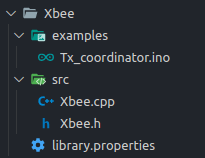
\includegraphics[scale=1]{xbee_lib.png}
\caption{ساختار فایل کتابخانه ایکس‌بی}\label{fig:xbee_lib}
\end{figure}

\subsubsection{ساختار فریم \lr{API}}

ساختار کلی فریم \lr{API} در \cref{fig:xbee_frame} \cite{Digi} نشان داده شده است. فریم با یک بایت جداکننده شروع می‌شود، سپس با ۲ بایت برای نشان‌دادن طول فریم ادامه می‌یابد و با یک بایت چک‌سام پایان می‌یابد. بایت‌های بین طول و فیلد چک‌سام را داده‌های فریم می‌نامند که برای هر نوع بسته \lr{API} متفاوت است. بایت اول فیلد طول مهم‌ترین بایت\LTRfootnote{Most Significant Byte(MSB)} و بایت بعدی کم‌اهمیت‌ترین\LTRfootnote{Least Significant Byte(LSB)} است. اولین بایت از داده‌های فریم نشان‌دهنده نوع فریم است. چک‌سام برای کمک به تست یکپارچگی داده‌ها استفاده می‌شود. اگر مقدار چک‌سام به اشتباه محاسبه شده‌باشد یا با چک‌سام واقعی داده‌های درون فریم متفاوت باشد، فریم کنار گذاشته و نادیده گرفته می‌شود.


\begin{figure}[!h]
\centering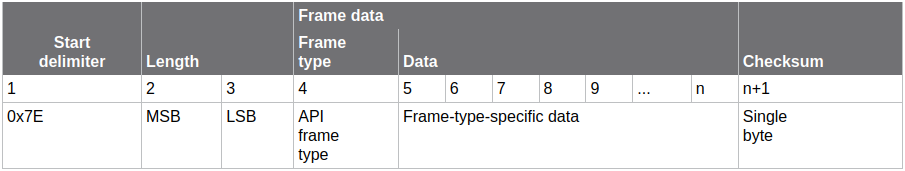
\includegraphics[scale=.65]{xbee_frame.png}
\caption{ساختار کلی فریم \lr{API} \cite{Digi}}\label{fig:xbee_frame}
\end{figure}

روش صحیح محاسبه چک‌سام فریم به شرح زیر است:
\begin{enumerate}
\item تمام بایت‌های بسته به استثنای محدودکننده شروع و طول با هم جمع می‌شوند.
\item از نتیجه فقط پایین‌ترین ۸ بیت نگه داشته می‌شود.
\item مقدار بدست‌آمده از \lr{0xFF} کم می‌شود.
\end{enumerate}

\subsubsection{فریم درخواست ارسال} \label{tx_req}

فریم‌های \lr{API} بسته به عملکردشان از چندین نوع فریم پشتیبانی می‌کنند. در این بخش فقط در مورد فریم درخواست ارسال که برای ما مهم است صحبت خواهیم کرد.

بخش‌های مختلف داده‌های فریم درخواست ارسال در \cref{tab:tx_req_frame} به همراه کاربرد آمده است.

\begin{table}[h!]
  \begin{center}
    \caption{بخش‌های مختلف داده‌های فریم درخواست ارسال \cite{Digi}}
    \label{tab:tx_req_frame}
    \begin{tabular}{|p{.1\textwidth}|p{.1\textwidth}|p{.25\textwidth}|p{.45\textwidth}|} % <-- Alignments: 1st column left, 2nd middle and 3rd right, with vertical lines in between
	   	\hline
	   	نام بخش & شماره بایت & نمونه & توضیحات\\
		\hline
	   	نوع فریم & ۳ & \lr{0x10} & بایت \lr{0x10} نشان‌دهنده فریم درخواست ارسال است.\\
		\hline
	   		   	شماره فریم & ۴ & \lr{0x01} & فریم داده را به گیرنده برای ارسال فریم وضعیت ارسال می‌شناساند. تنظیم‌کردن با مقدار ۰ پاسخ را غیرفعال می‌کند.\\
	    \hline
	   	آدرس ۶۴ بیتی مقصد & ۵ تا ۱۲ & \lr{0x0000000000000000} & آدرس ۶۴ بیتی مقصد را مشخص می‌کند.
	   	
 آدرس مقاصد خاص:
 
 	   	هماهنگ‌کننده: \lr{0x0000000000000000}
 	   	
همه‌پخشی\LTRfootnote{Broadcast}: \lr{0x000000000000FFFF}  	

نامعلوم(اگر آدرس مقصد را ندانیم): \lr{0xFFFFFFFFFFFFFFFF}
	   	\\
		\hline
	   	 	آدرس ۱۶ بیتی مقصد & ۵ تا ۱۲ & \lr{0x0000} & آدرس ۱۶ بیتی مقصد را مشخص می‌کند.
	   	
 آدرس مقاصد خاص:
 
 	   	هماهنگ‌کننده: \lr{0x0000}
 	   	

نامعلوم یا همه‌پخشی: \lr{0xFFFE}
	   	\\
		\hline
		شعاع پخش & ۱۵ & \lr{0x00} & حداکثر تعداد پرش‌هایی که انتقال همه‌پخشی می‌تواند پخش شود را تنظیم می‌کند. اگر روی ۰ تنظیم شود، شعاع پخش روی حداکثر مقدار پرش تنظیم می‌شود.\\
		\hline
		انتخاب‌ها & ۱۶ & \lr{0x00} & گزینه‌های انتقال پشتیبانی‌شده:

غیرفعال‌کردن تلاش ارسال مجدد - \lr{0x01}		

فعال‌کردن رمزگذاری \lr{APS}(با این کار حداکثر بایت‌های داده ارسالی تا ۴ بایت کاهش می‌یابد) - \lr{0x20}

استفاده از مهلت زمان طولانی برای ارسال - \lr{0x40}
		\\
		\hline
		داده ارسالی & ۱۷ به بعد & \lr{0x...} & تا ۲۵۵ بایت داده ارسالی برای مقصد\\
    	\hline
    \end{tabular}
  \end{center}
\end{table}

\subsubsection{داده ارسالی}

برای استفاده بهینه از فضای پیام در هر فریم، تصمیم گرفتیم ارتعاشات حسگر را به صورت زیر ارسال کنیم:

\begin{itemize}
\item هر داده با دقت ۳ رقم اعشار ارسال می‌شود.
\item برای جداسازی ارتعاش بر اساس محور در پیام ارسالی، از حروف \lr{x}، \lr{y} و \lr{z} استفاده نمی‌کنیم.
\item اولین بایت همیشه شناسه اندازه‌گیری را نشان می‌دهد. پس از آن پنج بایت اول نشان‌دهنده محور ایکس، پنج بایت بعدی نشان‌دهنده محور وای و پنج بایت بعدی نشان‌دهنده محور زد است. هر داده در پنج بایت نمایش داده می‌شود، برای مثال عدد ۴۵۲/۳- بصورت \lr{\{'-','3','4','5','2'\}} نمایش داده می‌شود.
\end{itemize}

در سمت گیرنده، داده‌ها باید به حالت اولیه تبدیل شوند.

\subsubsection{فایل \lr{Xbee.cpp} و توابع مهم}

برای تنظیم آدرس مقصد برای هر فریم کلاس \lr{XbeeDestAddress} را تعریف کرده‌ایم. این کلاس شامل فیلد ۶۴ بیتی و ۱۶ بیتی برای آدرس است. با توجه به اینکه به آرایه‌ای از بایت‌ها برای تشکیل فریم نیاز داریم، توابعی متناظر برای گرفتن هر یک از فیلدها نیز نوشته شده است.


برای تشکیل فریم درخواست انتقال کلاس \lr{XbeeRequest} تعریف شده است. تابع \lr{constructFrame} برای ایجاد فریم با استفاده از شناسه فریم و داده مورد نظر نوشته شده است. این تابع فریم را طبق \cref{tx_req} ایجاد کزده و فریم تشکیل‌شده برگردانده می‌شود. با استفاده از تابع \lr{writeFrameToSerial} نیز می‌توان فریم تشکیل‌شده را بر روی درگاه سریال دلخواه نوشت.

\subsection{‫ﺧﻮﺍﺑﻴﺪﻥ‬ ‫ﻭ‬ ‫ﺑﻴﺪﺍﺭﺷﺪﻥ‬ ‫ﺩﺭ‬ ‫ﺑﺎﺯﻩ‬‌‫ﻫﺎی ‬‫ﺯﻣﺎﻧﻲ‬ ‫ﻣﺸﺨﺺ‬}

برای کاهش مصرف انرژی، حسگر تنها در زمان‌های مشخص لرزش را احساس می‌کند. در سایر زمان‌ها بورد آردوینو برای کاهش مصرف انرژی به خواب می‌رود. برای این کار از کتابخانه \lr{LowPower.h} استفاده می‌کنیم. با استفاده از تابع \lr{powerDown} آردوینو به خواب می‌رود. برای بیدارشدن در زمان مشخص، آردوینو از زمان‌بند داخلی خود\LTRfootnote{Watchdog Timer} استفاده می‌کند. اما این تایمر بعد از ۸ ثانیه سرریز شده و بورد بیدار می‌شود. برای زمان‌های بیشتر باید به محض بیدارشدن مجدد تا رسیدن به زمان مورد نظر، آن را مجددا به خواب ببریم. این کار در تابع \lr{longSleep} انجام شده است.

\section{دروازه}

در دروازه ما از زبان برنامه‌نویسی پایتون برای دریافت فریم‌های زیگبی، ذخیره‌کردن و ارسال داده‌ها به سرور مرکزی پس از رسیدن به آستانه استفاده می‌کنیم. ساختار پروژه دروازه در \cref{fig:gateway_structure} نشان داده شده است. در این بخش به بررسی هر یک از فایل ها می‌پردازیم.


\begin{figure}[!h]
\centering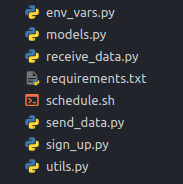
\includegraphics[scale=1]{gateway_structure.png}
\caption{ساختار پروژه دروازه}\label{fig:gateway_structure}
\end{figure}

\subsection{فایل \lr{env\_vars.py}}

این فایل از بسته \lr{load\_dotenv} برای خواندن متغیرهای محیطی استفاده می‌کند. برخی از این متغیرها برای برقراری ارتباط با سرور استفاده می‌شوند مانند شماره پورت سرور و آیپی سرور. سایر آنها برای برقراری ارتباط با دستگاه ایکس‌بی استفاده می‌شوند. این متغیرهای محیطی به عنوان متغیرهای پایتون تنظیم می‌شوند و سپس در ماژول‌های دیگر پایتون استفاده می‌شوند.

\subsection{فایل \lr{models.py}}

در این فایل ما سه کلاس برای نمایش داده‌های ارتعاش، اندازه گیری‌ها و هر گره انتهایی تعریف کرده‌ایم.

کلاس داده ارتعاش شامل داده‌های لرزش در سه محور ثبت‌شده توسط حسگر می‌باشد. هر اندازه‌گیری بسته به فرکانس نمونه‌برداری شامل چندین داده ارتعاش است. همچنین شامل یک شناسه و زمانی است که اندازه‌گیری در آن انجام شده است. از آنجایی که برای برقراری ارتباط داده‌های ارتعاش با زیگبی قطعه‌بندی\LTRfootnote{Fragmentation} لازم است و زمانی بین ارسال هر فریم لازم است، تابع \lr{thread\_handler} تعریف شده است تا در صورت اتمام زمان اتصال یا از بین رفتن برخی فریم‌ها، اندازه‌گیری از داده‌های دریافتی قبلی بطور خودکار تکمیل شود. پس از آن داده‌های جدید ذخیره می‌شوند.

هر گره دارای یک شناسه است که با شناسه فرستنده ارائه‌شده در هر فریم زیگبی مشخص می‌شود. همچنین هر گره شامل چندین اندازه‌گیری است. هنگامی که اندازه‌گیری جدیدی به لیست اندازه‌گیری‌ها اضافه می‌شود، زمان‌بند رشته‌ای\LTRfootnote{Thread Timer} با دوره وقفه مشخص و تابع \lr{thread\_handler} شروع می‌شود.

\subsection{فایل \lr{receiver.py}}

در این فایل سروری تعریف می‌کنیم که بطور بی‌نهایت به درگاه \lr{USB} متصل به دستگاه ایکس‌بی گوش می‌دهد. برای خواندن داده‌ها و استخراج داده هر فریم از کتابخانه \lr{digi-xbee} استفاده می‌کنیم. برای مقداردهی اولیه یک نمونه ایکس‌بی، درگاه و نرخ باود\LTRfootnote{Buad Rate} ارتباط لازم است. در تابع \lr{decode\_sensor\_data}، شناسه اندازه‌گیری و داده‌های ارتعاش را استخراج می‌کنیم. در تابع \lr{receive}، به منتظر دریافت پیام جدید می‌مانیم. داده‌های پیام را به گره و اندازه‌گیری مربوطه اضافه می‌کنیم و سپس داده‌های ذخیره‌شده را بروز می‌کنیم.

\subsection{فایل \lr{requirements.txt}}

این فایل برای تعیین بسته‌ها، نسخه‌ها و وابستگی‌های لازم استفاده می‌شود. سپس از این فایل برای نصب بسته‌های مشخص‌شده با مدیریت بسته پایتون پیپ\LTRfootnote{pip} استفاده می‌شود.

\subsection{فایل \lr{schedule.sh}}

آستانه تعریف‌شده بر اساس زمان است. این اسکریپت در کنار گیرنده اجرا می‌شود. در این اسکریپت یک کار \lr{crontab} برنامه‌ریزی می‌شود که هر ۱۵ دقیقه اجرا شود. این زمان‌بندی با استفاده از علامت \lr{*/15 * * * *} انجام می‌شود که به معنای اجرای اسکریپت ارسال داده پایتون در هر دقیقه قابل‌تقسیم بر ۱۵ است.

\subsection{فایل \lr{send\_data.py}}

در این فایل اطلاعات ذخیره‌شده در حافظه بارگذاری می‌شود. برای سرور و فراخوانی نقاط انتهایی \lr{API} از کتابخانه \lr{requests} استفاده می‌کنیم. برای دریافت رمز احراز هویت \lr{JWT} برای ارسال داده‌های ارتعاشی، یک درخواست پست با آدرس مک دستگاه و رمز عبور به سرور ارسال می‌شود تا رمز احراز هویت را دریافت کند. پس از آن داده‌های لرزش فرمت‌شده بصورت جیسان\LTRfootnote{JavaScript Object Notation(JSON)} در بدنه درخواست به همراه هدر احراز هویت به سرور ارسال و فایل ذخیره نیز پاک می‌شود.

\subsection{فایل \lr{signup.py}}

این فایل برای ثبت دروازه در سرور با رمز عبور و آدرس مک مربوطه استفاده می‌شود.

\subsection{فایل \lr{utils.py}}

این فایل شامل برخی از توابع کاربردی مانند دریافت آدرس مک دستگاه، دریافت زمان جاری در شکل مورد نظر، بروز رسانی داده‌های ذخیره‌شده و تعریف کلاس مدل جیسان برای کد‌کردن داده‌ها می‌باشد.

\section{پیش‌پردازش}

داده‌های جمع‌آوری‌شده از حسگر در هر سه محور می‌توانند تحت تاثیر شتاب گرانش زمین باشند. همچنین شتاب اندازه‌گیری‌شده توسط حسگرهای کم‌هزینه \lr{MEMS} نیز اکثرا تحت تاثیر یک مقدار غیرصفر دچار انحرافاتی می‌شوند که منجر به افزایش یا کاهش اندازه‌گیری‌ها می‌شود\cite{jung2017vibration}. برای حذف انحرافات و شتاب گرانش ناخواسته، داده‌ها را در مرحله پیش‌پردازش هنجارسازی می‌کنیم. برای حذف ناهنجاری‌ها مطابق \cref{form:norm} میانگین هر محور را از هر داده کم می‌کنیم. لازم به ذکر است که $\hat{a}^l_{nm}$ نماد ماتریس هنجارشده برای شتاب در سه محور، گره \lr{n} و اندازه‌گیری \lr{m}ام است.

\begin{equation}
\label{form:norm}
\hat{a}^l_{nm}=a^l_{nm}-\sum_{k=1}^K \dfrac{a^l_{nmk}}{K}
\end{equation}

\section{پایگاه داده سری زمانی}

مدل داده \lr{InfluxDB} داده‌های سری زمانی را در سطل‌ها\LTRfootnote{Buckets} و اندازه‌گیری‌ها سازماندهی می‌کند. یک سطل می‌تواند چندین اندازه‌گیری داشته باشد. اندازه‌گیری گروه‌بندی منطقی برای داده‌های سری زمانی است که شامل چندین برچسب\LTRfootnote{Tag} و فیلد است. همه نقاط در یک اندازه‌گیری معین باید برچسب‌های یکسانی داشته باشند. برچسب‌ها جفت‌های کلید-مقدار با مقادیری متفاوت هستند که اغلب تغییر نمی‌کنند و برای ذخیره ابرداده\LTRfootnote{Meta data} برای هر نقطه در نظر گرفته شده‌اند. فیلدها جفت‌های کلید-مقدار هستند که مقادیر آنها در طول زمان تغییر می‌کنند. زمان مرتبط با داده‌ها نیز ذخیره می‌شوند و هنگام پرس‌وجو داده‌ها برحسب آن مرتب می‌شوند\cite{influx_doc}.


برای ارتباط با پایگاه داده از کلاینت پایتون \lr{influxDB} استفاده می‌کنیم. برای شروع یک اتصال به نام سطل، سازمان، نشانه و نشانی نیاز داریم. برای نوشتن داده‌ها از تابع \lr{write\_api} و برای پرس‌وجوی داده‌ها در پایگاه داده از \lr{query\_api} استفاده می‌کنیم.


برای نوشتن داده‌ها باید نقاطی را که می‌خواهیم اضافه کنیم، مشخص کنیم. نقطه یک داده واحد است که با اندازه‌گیری، کلیدهای برچسب، مقادیر برچسب، کلید فیلد و زمان مشخص می‌شود. برای پرس‌وجوی داده‌ها، از عملگر لوله جلو\LTRfootnote{Pipe-Forward(|>)} برای اتصال خروجی یک تابع بعنوان ورودی تابع بعدی استفاده می‌کند\cite{influx_doc}. سه تابع اصلی برای پرس‌وجوکردن داده‌ها وجود دارد:

\begin{itemize}
\item \lr{from()}: داده‌ها را از یک سطل جستجو می‌کند.
\item \lr{range()}: داده‌ها را بر اساس محدوده‌ی زمانی فیلتر می‌کند. برای جستجو به پرس‌وجوهای محدود به یک بازه‌ی زمانی خاص نیاز داریم.
\item \lr{filter()}: داده‌ها را بر اساس مقادیر ستون فیلتر می‌کند. هر سطر با \lr{r} و هر ستون با ویژگی \lr{r} نشان داده می‌شود. می‌توان چند فیلتر متوالی اعمال کرد.
\end{itemize}

تابع دیگری که استفاده کرده‌ایم \lr{pivot()} است که برای تبدیل داده‌ها به یک طرح رابطه‌ای\LTRfootnote{Relational Schema} بر اساس زمان استفاده می‌شود.

\subsection{ساختار کلی}

ساختار کلی پایگاه داده طراحی‌شده در این پروژه در \cref{fig:influx_structure} نشان داده شده است. هر یک از ویژگی‌های استخراج‌شده در سمت چپ در اندازه‌گیری‌های مختلف قرار گرفته‌اند. در وسط تصویر نیز برچسب‌ها که بین همه اندازه‌گیری‌ها مشترک است قرار گرفته است. در سمت راست تصویر نیز فیلدهای هر اندازه‌گیری آورده شده است. در ادامه به توضیح توابع نوشتن و پرس‌وجوی اندازه‌گیری‌ها می‌پردازیم.


\begin{figure}[!h]
\centering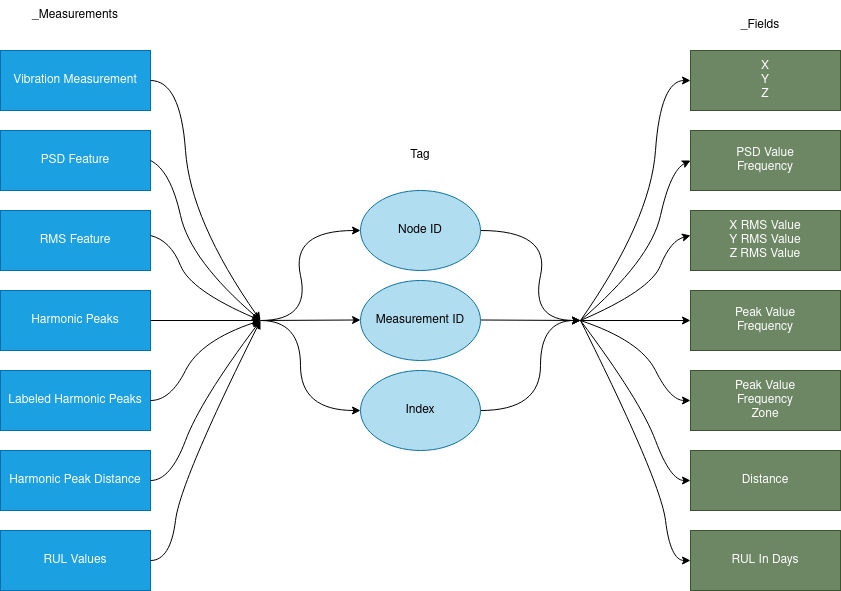
\includegraphics[scale=.5]{influx_structure.png}
\caption{ساختار کلی پایگاه داده سری زمانی}\label{fig:influx_structure}
\end{figure}

\subsection{اندازه‌گیری‌ها و توابع مربوط به نوشتن و گرفتن داده}

در هر اندازه‌گیری، فیلدهای مربوط را ذخیره می‌کنیم. فیلدهای هر داده ثبت می‌شود و با یک گره و یک اندازه‌گیری همراه است. همچنین یک شماره به هر نمونه در اندازه‌گیری بعنوان شناسه داده می‌شود.

برای نوشتن داده‌ها در پایگاه داده توابع \lr{write\_\$\{measurement name\}} پیاده‌سازی شده است که یک نقطه جدید برای هر داده با شناسه اندازه‌گیری، شناسه گره و شماره بعنوان برچسب و فیلدهای مربوطه ایجاد می‌کند.

برای پرس‌وجوی داده، توابع \lr{get\_\$\{measurement name\}} پیاده‌سازی شده است. پرس‌وجو بگونه‌ای نوشته شده است که اگر شناسه اندازه‌گیری یا شناسه گره ارائه شود، فقط داده‌های مرتبط برگردانده می‌شود. در هر پرس‌وجو، ما تمام داده‌ها را از اندازه‌گیری مربوط انتخاب می‌کنیم و در صورت وجود شناسه گره یا اندازه‌گیری فیلتر می‌کنیم. سپس زمان فیلدها، مقادیر آنها و برچسب‌ها را نگه می‌داریم و از تابع \lr{pivot} برای تبدیل نتایج به طرح رابطه‌ای استفاده می‌کنیم. بعنوان نمونه، کد پرس‌وجوی \lr{vibration\_measurement} در \cref{fig:vm_query} نشان داده شده است.

\begin{figure}[!h]
\centering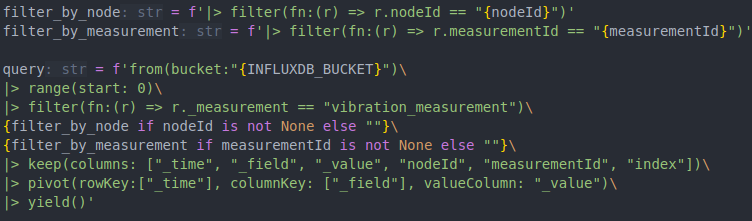
\includegraphics[scale=.75]{vm_query.png}
\caption{کد پرس‌وجوی \lr{vibration\_measurement}}\label{fig:vm_query}
\end{figure}

\subsection{توابع گرفتن شناسه گره و اندازه‌گیری}

در این توابع برای گرفتن شناسه‌ها به تنهایی، برچسب مورد نظر را نگه می‌داریم و جهت جلوگیری از تکرار با استفاده از تابع \lr{unique()} مقادیر یکتای شناسه را برمی‌گردانیم.

\subsection{تابع \lr{get\_starting\_service\_date}}

این تابع برای دریافت زمان اولین داده ثبت‌شده بعنوان مبدا زمانی برای محاسبه زمان سرویس‌شدن تجهیزات نوشته شده است.

\subsection{تابع حذف داده‌ها و حافظه پنهان}

برای حذف از کلاس \lr{DeleteApi} کتابخانه استفاده می‌کنیم. جهت حذف حافظه پنهان، همه اندازه‌گیری‌ها را، بجز آنهایی که خودمان تعریف کرده‌ایم، تا زمان فعلی حذف می‌کنیم. همچنین برای حذف همه داده‌ها با استفاده از تابع \lr{clear\_vibration\_data}، همه اندازه‌گیری‌ها را حذف می‌کنیم.

\section{برنامه وب و چارچوب ویو}

وظایف مختلفی در توسعه‌ی یک برنامه وب سمت کاربر وجود دارد. بسته‌های زیادی برای بخشی خاص توسعه داده شده‌اند تا کار توسعه برنامه آسان‌تر شود. در این پروژه علاوه بر استفاده از چارچوب ویو، از کتابخانه‌ها و ماژول‌های دیگر برای کارهای مختلف استفاده کرده‌ایم. در این قسمت در مورد کتابخانه‌های مهم استفاده‌شده، ساختار فایل پروژه و اجزای اصلی برنامه صحبت و تصاویری از محیط پیاده‌سازی‌شده را مشاهده می‌کنیم.

\subsection{کتابخانه‌ها و ماژول‌ها}

\subsubsection{چارچوب ناکست}

ناکست\LTRfootnote{Nuxt} یک چارچوب توسعه وب سطح بالای نودجی‌اس\LTRfootnote{Node.js} برای ایجاد برنامه‌های ویو است که می‌تواند در دو حالت مختلف برنامه جهانی\LTRfootnote{Universal(SSR)} و تک‌صفحه‌ای\LTRfootnote{Single Page Application(SPA)} توسعه و استقرار یابد. علاوه بر این، می‌توان این دو نوع را در ناکست بعنوان برنامه‌های تولیدشده ایستا\LTRfootnote{Static} مستقر کرد. قدرت کامل ناکست در حالت جهانی یا تفسیر سمت سرور نهفته است. ناکست بر روی ویو ایجاد شده است و دارای ویژگی‌های اضافی مانند داده‌های ناهمزمان، میان‌افزار، طرح‌بندی، ماژول‌ها و افزونه‌ها است که برنامه را ابتدا در سمت سرور و سپس در سمت کلاینت اجرا می‌کند. در این حالت برنامه معمولاً سریع‌تر از برنامه‌های سنتی سمت سرور ارائه می‌شود\cite{kok2020hands}. ناکست ساختار فایل ساده‌ای نیز دارد که توسعه برنامه وب را بسیار ساده‌تر می‌کند که در بخش بعدی در مورد آن توضیح می‌دهیم.


\subsubsection{کتابخانه ویوتیفای}

ویوتیفای\LTRfootnote{Vuetify} یک چارچوب کامل رابط کاربری است که بر روی ویو ساخته شده است. هدف این پروژه ارائه ابزارهای مورد نیاز توسعه‌دهندگان برای ایجاد تجربیات کاربر غنی و جذاب است. برخلاف سایر چارچوب‌ها، ویوتیفای از ابتدا به گونه‌ای طراحی شده است که یادگیری آن آسان است و صدها مؤلفه با دقت ساخته‌شده از مشخصات طراحی مادی\LTRfootnote{Material Design} همراه آن است\cite{vuetify}.

ویوتیفای برای طراحی از یک رویکرد اول تلفن همراه\LTRfootnote{Mobile First} استفاده می‌کند، به این معنی که برنامه وب به‌سادگی و بدون بهم‌ریختگی روی تلفن همراه، تبلت یا رایانه اجرا می‌شود. ویوتیفای را می‌توان به‌سادگی بعنوان یک ماژول به ناکست اضافه و در پروژه استفاده کرد\cite{vuetify}.


\subsubsection{کتابخانه چارت}

در ابن پروژه چندین داده تحلیلی داریم که با استفاده از نمودارها قابل مشاهده هستند. برای این کار از کتابخانه چارت‌\LTRfootnote{Chart.js} استفاده کرده‌ایم. کتابخانه چارت مجموعه‌ای از انواع نمودارها، افزونه‌ها و گزینه‌های سفارشی‌سازی را ارائه می‌دهد. علاوه بر مجموعه‌ای معقول از انواع نمودار داخل کتابخانه، می‌توان از انواع نمودارهای توسعه‌داده‌شده توسط جامعه نیز استفاده کرد. علاوه بر این، می‌توان چندین نوع نمودار را در یک نمودار ترکیبی قرار داد. این کتابخانه با افزونه‌های سفارشی ایجاد حاشیه‌نویسی، بزرگنمایی یا قابلیت کشیدن و رهاکردن را ممکن ساخته است\cite{chart}.

\subsubsection{کتابخانه اکسیوس}

اکسیوس\LTRfootnote{Axios} یک سرویس گیرنده \lr{HTTP} مبتنی بر وعده\LTRfootnote{Promise} برای نودجی‌اس و مرورگر است که می‌تواند در هر دو با پایگاه کد مشابه اجرا شود. این کتابخانه در سمت سرور از ماژول اصلی \lr{HTTP} نودجی‌اس و در مرورگر از \lr{XMLHttpRequests} استفاده می‌کند. مزیت اصلی این کتابخانه سادگی در ارسال درخواست‌های مختلف، دریافت پاسخ آنها و پشتیبانی از \lr{API} وعده است\cite{axios}. همچنین می‌توان آن را بعنوان یک ماژول به پروژه ناکست اضافه کرد.

\subsubsection{ماژول احراز هویت ناکست}

احراز هویت بخش بسیار مهمی از هر برنامه وب است که شامل مراحل زیر است:

\begin{itemize}
\item ارسال اطلاعات کاربران به سرور جهت تایید
\item دریافت و ذخیره توکن احراز هویت
\item استفاده از آن توکن برای تماس های بعدی \lr{API}
\end{itemize}

این ماژول با استفاده از یک طرح احراز هویت قابل‌تنظیم یا با استفاده از یکی از ارائه‌دهندگان مستقیم پشتیبانی‌شده، احراز هویت کاربران را تأیید می‌کند و یک \lr{API} برای احراز هویت و دسترسی به اطلاعات کاربر فراهم می‌کند. در حالیکه این ماژول ذخیره اطلاعات در سمت کاربر را بر عهده دارد، مدیریت جلسه یا احراز هویت مبتنی بر جلسه در سمت سرور را ارائه نمی‌کند\cite{nuxt_auth}.

\subsection{ساختار پروژه}

ساختار پروژه در \cref{fig:front_structure} نشان داده شده است. برخی از فایل‌ها و پوشه‌ها بخشی از چارچوب ناکست هستند.

\begin{figure}[!h]
\centering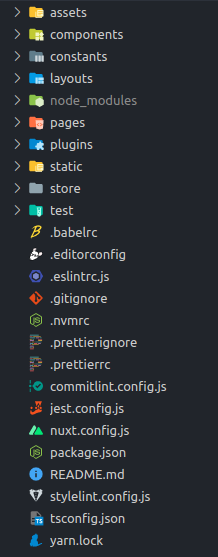
\includegraphics[scale=.75]{front_structure.png}
\caption{ساختار پروژه برنامه وب}\label{fig:front_structure}
\end{figure}

برخی دیگر از این فایل‌ها مانند \lr{eslint} برای هشدار در مواقعی که کد نوشته‌شده مطابق قواعد تعریف شده نباشد استفاده می‌شود، برخی دیگر مانند \lr{style lint} برای داشتن سبکی یکپارچه و تمیز در بین همه فایل‌ها و توسعه‌دهندگان استفاده می‌شوند.

همچنین چند فایل وجود دارد که بسته‌های لازم، نسخه‌های آنها و همچنین چند اسکریپت برای اجرای پروژه را مشخص می‌کنند. مدیریت‌کننده بسته مورد استفاده در این پروژه یارن\LTRfootnote{Yarn} نام دارد. در فایل \lr{yarn.lock} نسخه‌های دقیق بسته‌ها و وابستگی‌های آنها توسط یارن مشخص شده است و از آن برای سریع و قابل‌اعتمادبودن تفکیک وابستگی‌ها استفاده می‌کند. در فایل \lr{package.json} اسکریپت‌ها، وابستگی‌ها و وابستگی‌های زمان توسعه مشخص شده‌اند. این فایل برای شناسایی بسته‌های لازم توسط یارن در اولین اجرا لازم است.

\subsubsection{پوشه \lr{assets}}

این پوشه شامل فایل‌های تفسیرنشده مثل استایل‌ها\LTRfootnote{Styles}، تصاویر و فونت‌ها است\cite{nuxt}.

\subsubsection{پوشه \lr{components}}

این پوشه حاوی مؤلفه‌های ویو است. مؤلفه‌ها بخش‌های مختلف صفحه را تشکیل می‌دهند و می‌توانند دوباره استفاده شوند و در صفحات، طرح‌بندی‌ها\LTRfootnote{Layouts} و حتی سایر مؤلفه‌ها قرار گیرند\cite{nuxt}.

\subsubsection{پوشه \lr{layouts}}

برای تغییر ظاهر برنامه، طرح‌بندی‌ها کمک بزرگی هستند. این تغییر می‌تواند افزودن نوار کناری\LTRfootnote{Sidebar} یا طرح‌بندی‌های متفاوت برای تلفن‌همراه و رایانه باشد. در این پروژه دو طرح‌بندی پیش‌فرض و خطا وجود دارد\cite{nuxt}.

\subsubsection{پوشه \lr{pages}}

این پوشه شامل نماها و مسیرهای برنامه است. ناکست تمام فایل‌های \lr{.vue} داخل این پوشه را می‌خواند و بطور خودکار پیکربندی مسیریاب را ایجاد می‌کند\cite{nuxt}.

\subsubsection{پوشه \lr{plugins}}

این پوشه شامل افزونه‌های جاوا اسکریپت است که می‌خواهیم قبل از نمونه‌سازی ریشه برنامه اجرا کنیم\cite{nuxt}. در این پروژه برای ایجاد مؤلفه نمودارها و همینطور دخالت در درخواست‌های اکسیوس و مدیریت خطاهای مربوط به آن افزونه‌هایی نوشته‌ایم.

\subsubsection{پوشه \lr{statics}}

این پوشه بطور مستقیم به ریشه سرور نگاشت می‌شود و حاوی فایل‌هایی است که تغییر نخواهند کرد. همه فایل‌های ارائه‌شده بطور خودکار توسط ناکست ارائه\LTRfootnote{Serve} می‌شوند و از طریق آدرس ریشه پروژه قابل دسترسی هستند\cite{nuxt}.

\subsubsection{پوشه \lr{store}}

گاهی اوقات در پروژه به اطلاعات مشترک و قابل دسترسی بین همه مؤلفه‌ها نیاز داریم. یکی از راهکارهای این مسئله استفاده از سیستم ذخیره‌سازی مرکزی است که در آن یک بخش داده‌های مشخص‌شده و تغییراتشان را مدیریت می‌کند. در ویو این مسئولیت بر عهده ویوایکس\LTRfootnote{Vuex} است. این پوشه شامل فایل‌های ویوایکس است. ویوایکس همراه ناکست و بصورت خارج از جعبه\LTRfootnote{Out of the Box} عرضه می‌شود اما بطور پیش‌فرض غیرفعال است. ایجاد یک فایل \lr{index.js} در این پوشه، ویوایکس را فعال می کند\cite{nuxt}. در این پروژه برای نگهداری مشخصات ظاهری و مدیریت ورود کاربران از ویوایکس استفاده می‌کنیم.

\subsubsection{فایل \lr{nuxt.config.js}}

بطور پیش‌فرض، ناکست برای پوشش بیشتر موارد استفاده پیکربندی شده است. این پیکربندی پیش‌فرض ناکست و ماژول‌های آن را می‌توان با فایل \lr{nuxt.config.js} بازنویسی کرد\cite{nuxt}. بازنویسی‌های ما شامل افزودن برچسب‌های ابرداده، مشخص‌کردن ماژول‌ها، افزودنی‌ها و استایل کلی و پیکربندی برخی ماژول‌ها مانند ماژول احراز هویت(برای مشخص‌کردن روش احراز هویت، مسیرهای حفاظت‌شده و آدرس سرور برای تاید احراز هویت) و ویوتیفای(برای مشخص‌کردن ظاهر صفحات و رنگ‌ها) است.

\subsection{مؤلفه‌های اصلی}

در این بخش در مورد اجزای اصلی و برخی از صفحات این پروژه صحبت خواهیم کرد.


\subsubsection{کارت خلاصه}

در این مؤلفه، آمار خلاصه همه موارد مختلف را نشان می‌دهیم. عنوان، خلاصه و نماد بعنوان ورودی\LTRfootnote{Props} ارائه می‌شوند و به‌سادگی با تکرار روی هر مورد نشان داده می‌شوند. نتایج را می‌توان در \cref{fig:summary_card} مشاهده کرد که آمار کاربران، گره‌ها و دروازه‌ها را نشان می‌دهد.

\begin{figure}[!h]
\centering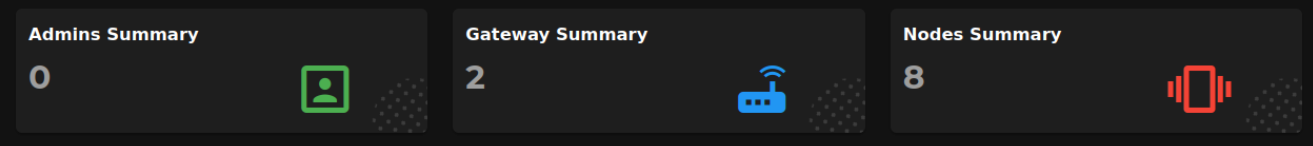
\includegraphics[scale=.45]{summary_card.png}
\caption{مؤلفه کارت خلاصه}\label{fig:summary_card}
\end{figure}

\subsubsection{فرم‌ها}

تمامی اجزای مربوط به فرم‌ها در این پوشه قرار دارند. مؤلفه ورود دارای دو فیلد متنی برای ایمیل و رمز عبور کاربران است. هنگامی که کاربر بر روی دکمه ورود کلیک می‌کند، معتبربودن ایمیل و رمز عبور بررسی می‌شود. سپس درخواست مجوز برای کاربر به سرور ارسال می‌شود و در صورت صحیح‌بودن اطلاعات، کاربر به صفحه اصلی هدایت می‌شود. در غیر این صورت، پیام خطای مناسب با مولفه اسنک‌یار\LTRfootnote{SnackBar} نمایش داده می‌شود. در \cref{fig:login_page} صفحه ورود با پیام خطای نادرستی رمز عبور نشان داده شده است.

\begin{figure}[!h]
\centering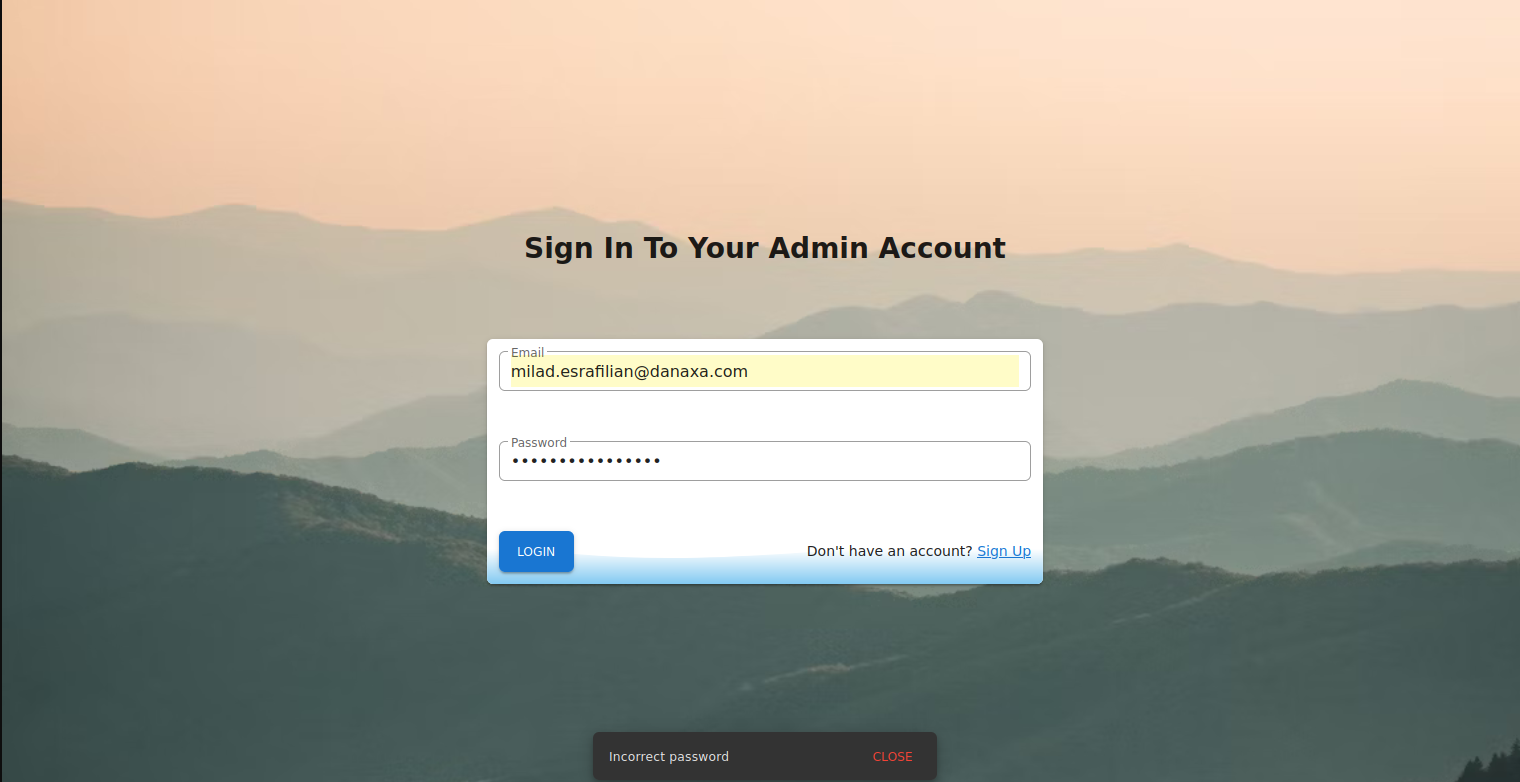
\includegraphics[scale=.38]{login_page.png}
\caption{صفحه ورود و پیغام خطای رمز عبور نادرست}\label{fig:login_page}
\end{figure}

همین روند در مؤلفه ثبت‌نام طی می‌شود، با این تفاوت که یک فیلد نام نیز در آن وجود دارد که در \cref{fig:signup_page} قابل مشاهده است.

\begin{figure}[!h]
\centering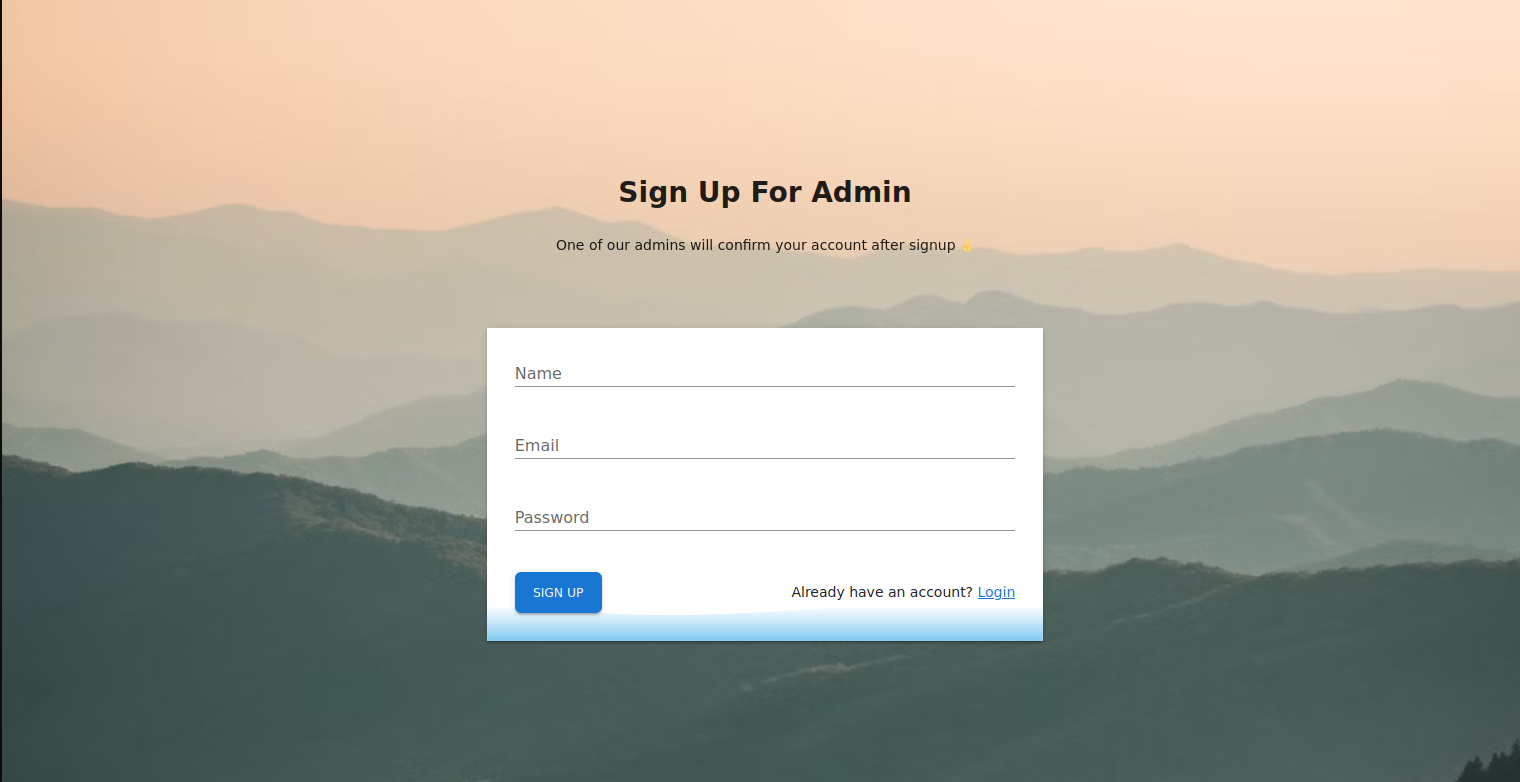
\includegraphics[scale=.38]{signup_page.png}
\caption{صفحه ثبت‌نام کاربر جدید}\label{fig:signup_page}
\end{figure}

\subsubsection{اسنک‌بار}

مؤلفه اسنک‌بار برای نمایش پیام‌های خطا استفاده می‌شود. پیغام خطا به عنوان ورودی به آن داده می‌شود. اسنک‌بار را می‌توان با فشردن دکمه بستن بست.


\subsubsection{فوتر}

فوتر\LTRfootnote{Footer} در پایین تمام صفحات نشان داده می‌شود و شامل تاریخ و پیام کپی‌رایت\LTRfootnote{Copy Right} است.

\subsubsection{مؤلفه‌های \lr{GatewayDetail} و \lr{UserDetail}}

این دو مولفه بسیار شبیه بهم هستند اما اطلاعات متفاوتی را درباره کاربران و دروازه‌ها نشان می‌دهند. هر کاربر و دروازه باید پس از ثبت‌نام توسط مدیر دیگری تایید شود. این کار را می‌توان با تغییر کلید تایید در صفحات مرتبط انجام داد. \cref{fig:gateway_page} دو دروازه فعال تاییدشده را نشان می‌دهد. پس از تایید کاربر یا دروازه، کلید غیرفعال می‌شود.

\begin{figure}[!h]
\centering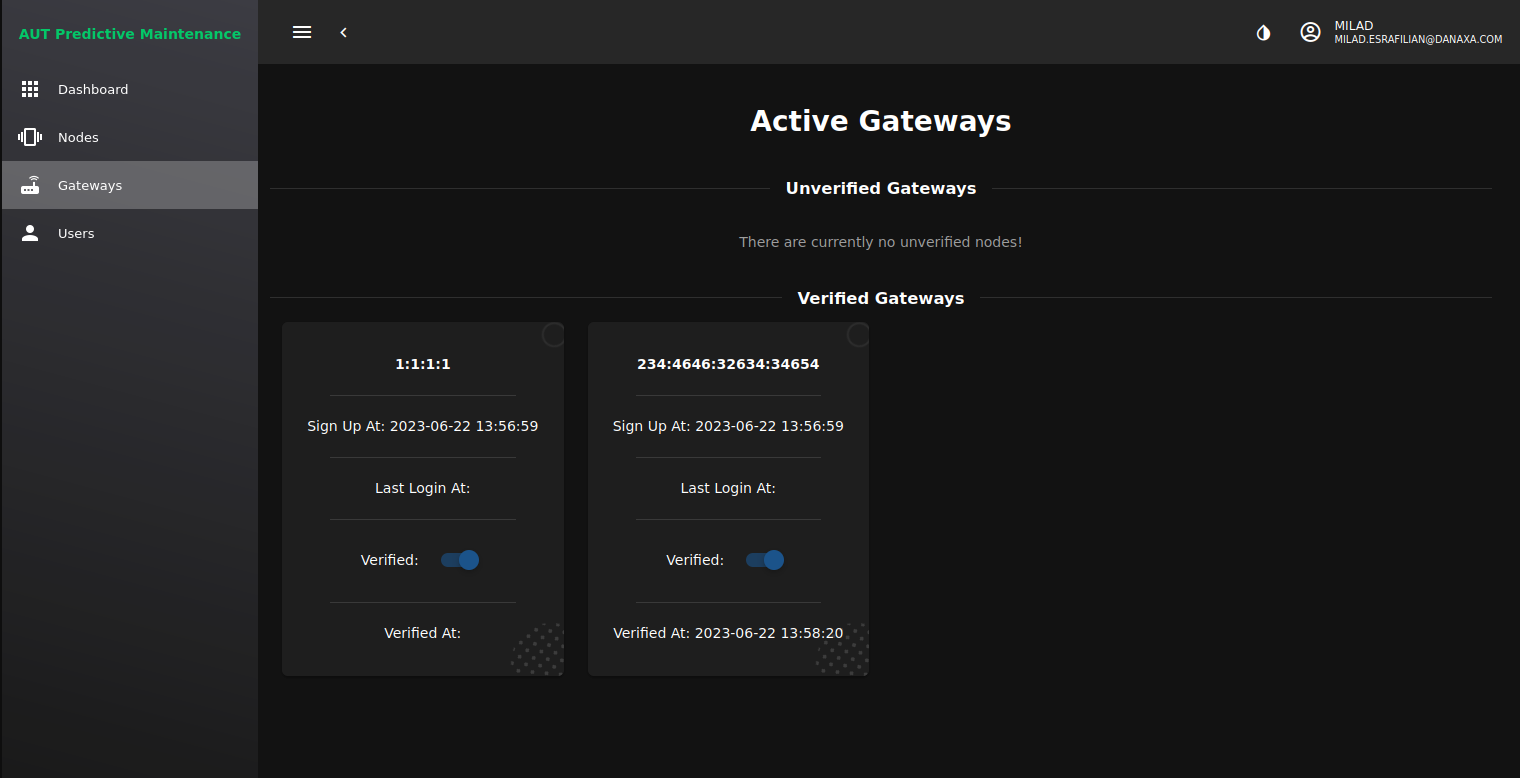
\includegraphics[scale=.38]{gateway_page.png}
\caption{صفحه دروازه‌های فعال}\label{fig:gateway_page}
\end{figure}

\subsubsection{داشبورد}

داشبورد\LTRfootnote{Dashboard} یک نمای کلی از ادمین‌های فعال، دروازه‌ها و گره‌ها ارائه می‌دهد. همچنین در این صفحه می‌توانیم به هر گره مطابق \cref{fig:dashboard} دسترسی داشته باشیم.

\begin{figure}[!h]
\centering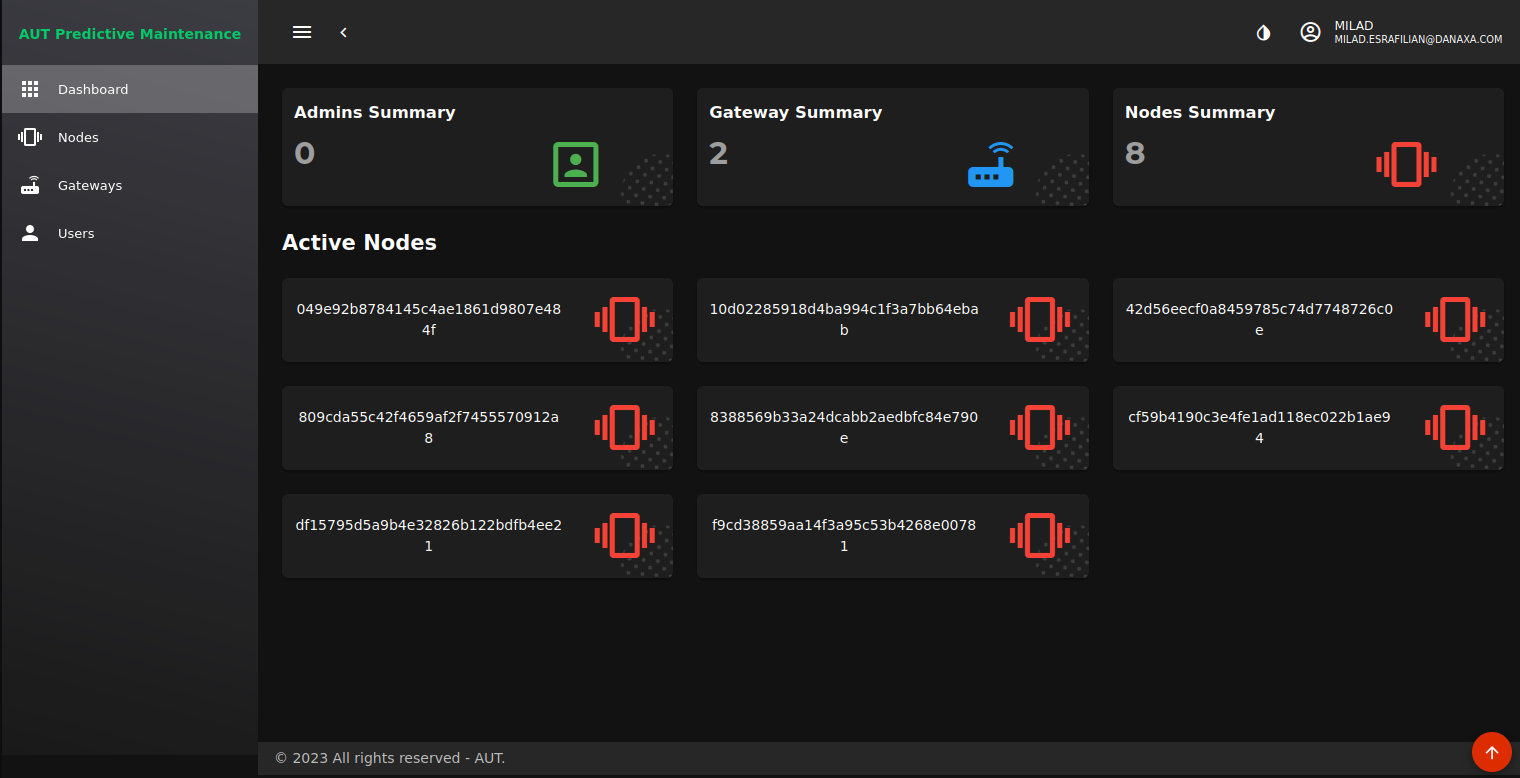
\includegraphics[scale=.38]{dashboard.png}
\caption{صفحه داشبورد}\label{fig:dashboard}
\end{figure}

\subsubsection{گره}

با کلیک بر روی هر گره، کاربر به صفحه گره مربوط هدایت می‌شود. همانطور که در \cref{fig:rms_chart} نشان داده شده است، سه برگه برای مشاهده نمودار تحلیلی مورد نظر وجود دارد. شکل انتخاب پیش‌فرض را نشان می‌دهد که ریشه میانگین مربع است. هنگامی که این صفحه بارگذاری می‌شود یا زمانی که برگه‌ها تغییر می‌کنند درخواستی به نقطه پایانی مناسب ارسال می‌شود و سپس نمودار مرتبط نشان داده می‌شود. برای نمایش نمودارها از افزونه چارت‌جی‌اس و نمودار خطی استفاده می‌کنیم.

\begin{figure}[!h]
\centering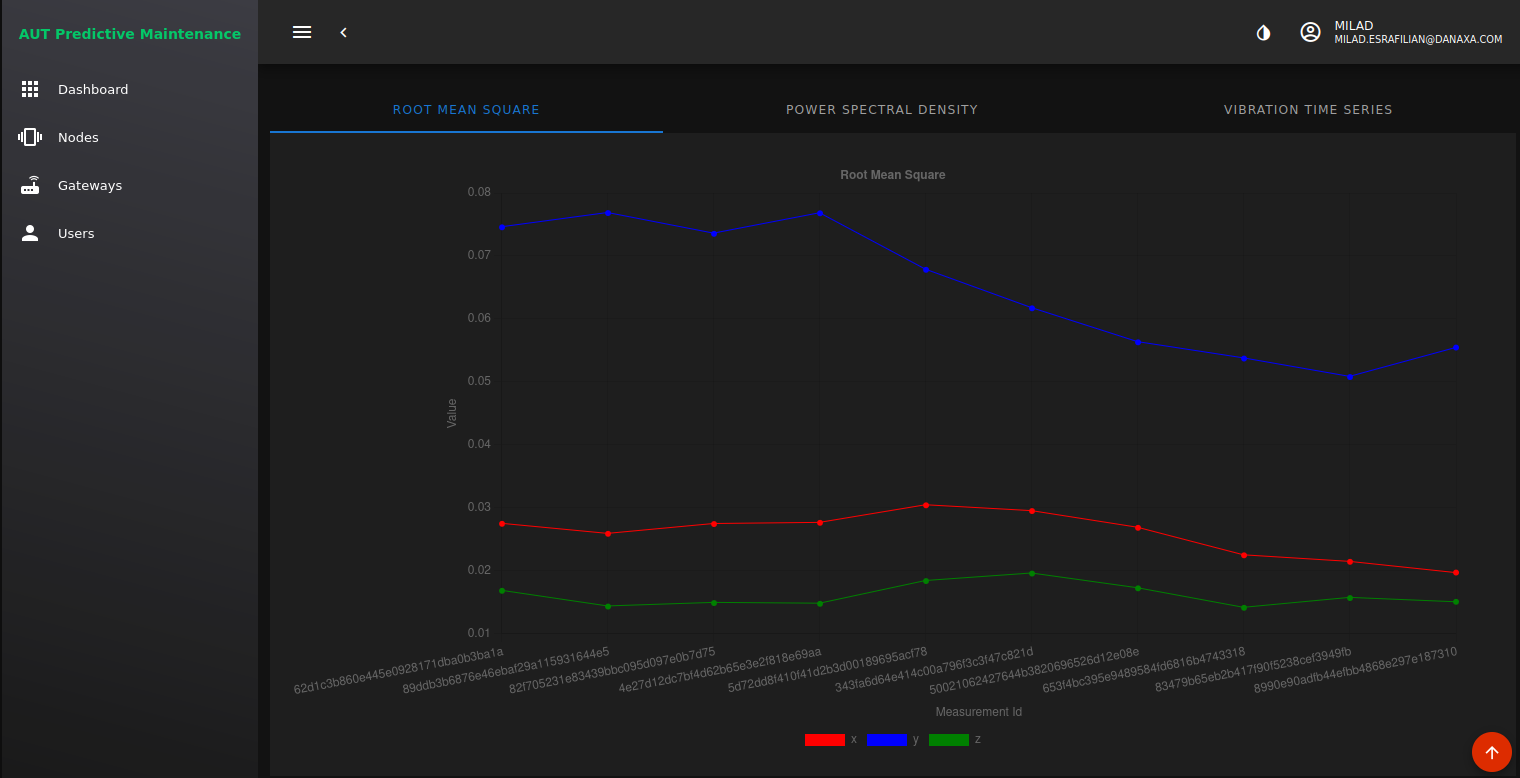
\includegraphics[scale=.38]{rms_chart.png}
\caption{نمودار ریشه میانگین مربع}\label{fig:rms_chart}
\end{figure}

برای نمایش نمودار چگالی طیفی توان، ابتدا شناسه اندازه‌گیری باید از ورودی کشویی انتخاب شود. پس از انتخاب، دو درخواست برای دریافت مقادیر \lr{PSD} و قله‌ها به سرور ارسال می‌شود. سپس قله‌ها مطابق \cref{fig:psd_chart} به همراه نمودار چگالی طیفی توان با نقاط بزرگ‌تر نشان داده می‌شوند.

\begin{figure}[!h]
\centering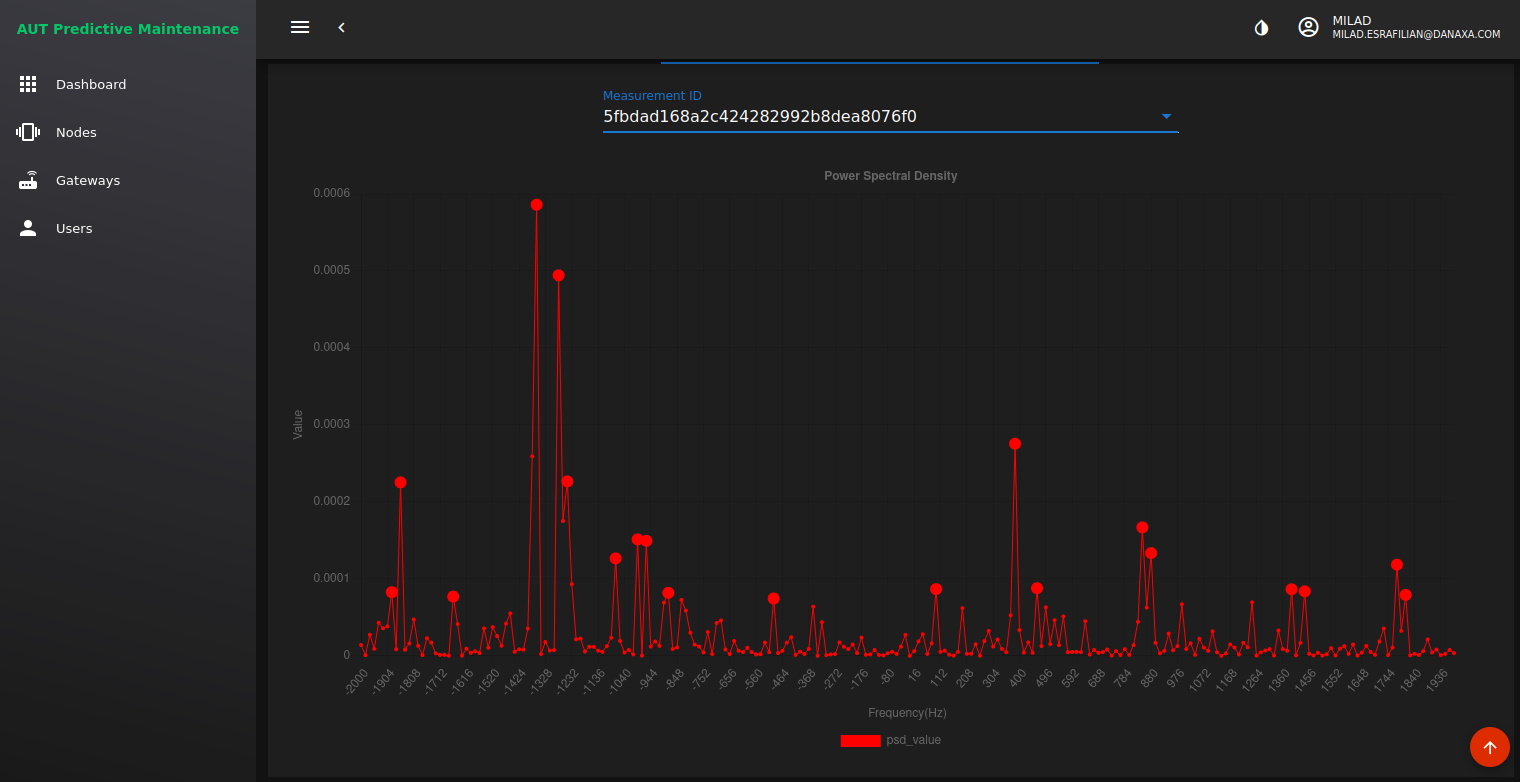
\includegraphics[scale=.38]{psd_chart.png}
\caption{نمودار چگالی طیفی توان}\label{fig:psd_chart}
\end{figure}

سری زمانی ارتعاش، داده‌های خام سه محور را مطابق \cref{fig:vdt_chart} در یک نمودار نشان داده می‌شود. در این برگه نیز لازم است ابتدا شناسه اندازه‌گیری انتخاب شود تا نمودار نمایش داده شود.

\begin{figure}[!h]
\centering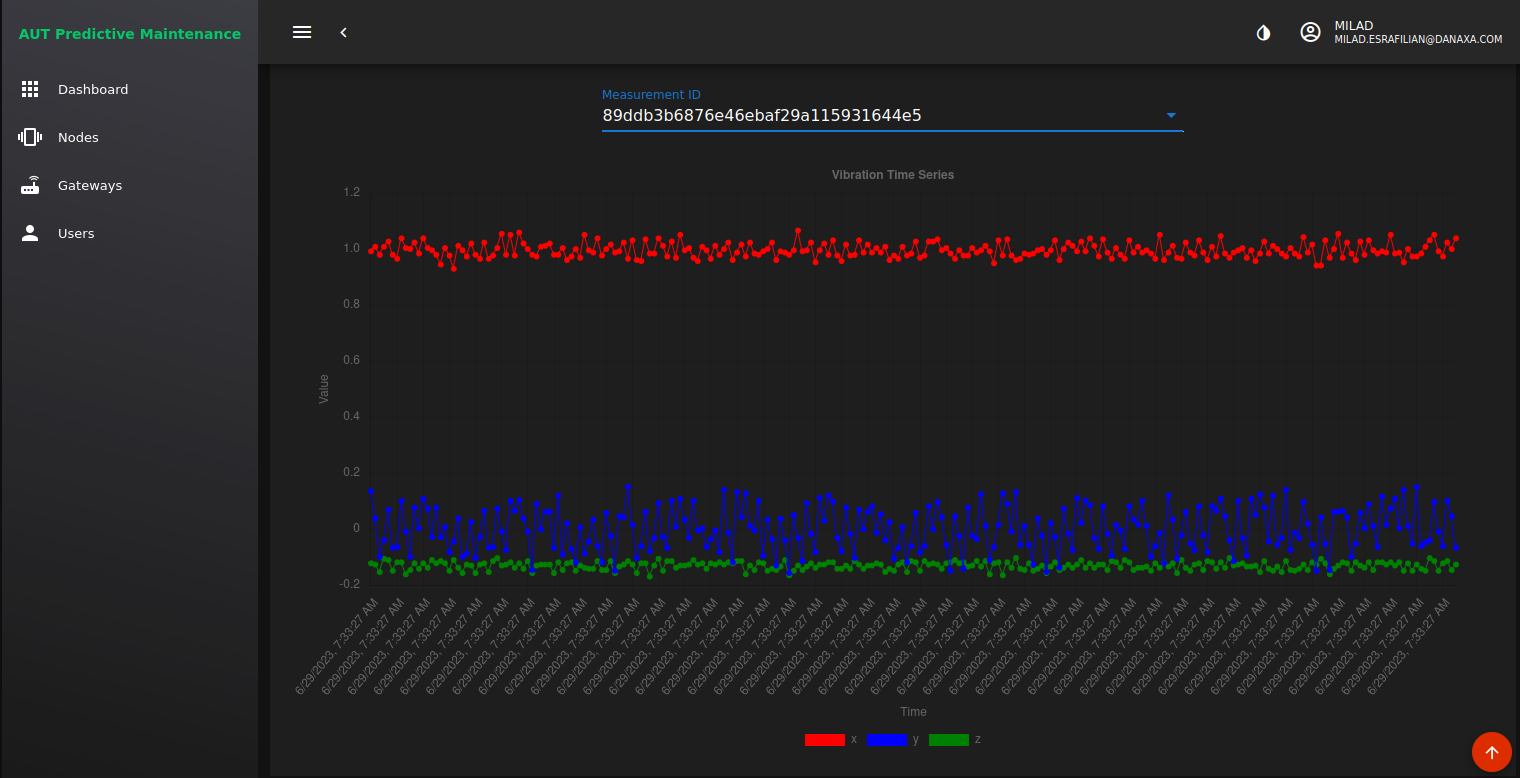
\includegraphics[scale=.38]{vdt_chart.png}
\caption{نمودار سری زمانی ارتعاش}\label{fig:vdt_chart}
\end{figure}

\section{نتیجه‌گیری و جمع‌بندی}

در این بخش در مورد نحوه پیاده‌سازی سیستم صحبت کردیم. ابتدا در مورد ساختار کلی سیستم صحبت کردیم، سپس در مورد نحوه پیاده سازی کد در آردوینو برای گره‌ها صحبت کردیم. سپس دروازه و تمام فایل‌های آن را توضیح دادیم. سپس در مورد پیش‌پردازش و هنجارسازی داده‌ها صحبت کردیم. پس از آن در مورد طرز کار و کتابخانه پایگاه داده سری زمانی برای نوشتن و چستجوی داده‌ها صحبت کردیم و در پایان در مورد برنامه وب و نحوه کار با آن صحبت کردیم و چند تصویر از خروجی را نیز نشان دادیم.

\chapter{مشخصات یک پایان نامه و گزارش علمی}

اگرچه براي همه انواع نوشته‌ها، مشخصات و ويژگي‌هاي واحد و معيني نمي‌توان ذكر كرد، با اين حال در یک پایان نامه یا گزارش علمی باید نکات و موارد کلی که در این فصل ذکر می‌شود، بطور کامل رعایت شده باشد. 

دقت كنيد كه پس از عنوان فصل بايد حداقل توضیحی کوتاه در مورد موضوع نوشته شود و نمي‌توان مستقيماً بعد از آن عنوان بخش را نوشت و همين طور پس از عناوين بخش‌ها و زيربخش‌ها.(مانند دستورالعمل حاضر)
\section{برخورداری از غنای علمی }

يك پایان نامه بايد پیش از هر چيز به‌لحاظ علمي از غناي لازم برخوردار باشد. يعني هدف و پيام روشني داشته باشد و از پيش‌زمينه علمي، بيان دلايل علمی، ارجاعات مورد نیاز و نتيجه‌گيري شفاف بهره ببرد. 

\section{ارجاع به‌موقع و صحیح به منابع دیگر}
هر جمله‌ای که در یک پایان نامه نوشته می‌شود یا یک جمله کاملاً بدیهی است یا باید دلیل آن بیان شود و یا اینکه باید به منبعی که آن موضوع را نقل یا اثبات کرده، ارجاع داده شود. اگر مطلب يا گفتاري از منبعی عيناً در گزارش نقل مي‌شود، بايد آن مطلب داخل گيومه قرار گيرد و با ذكر ماخذ و شماره صفحه، به آن اشاره گردد.


\section{ساده‌نویسی }
سادگی از ضروريات يك نوشته است. نويسنده بايد ساده، روان و در عين حال شيوا و رسا بنويسد و عبارات مبهم، جملات پيچيده و كلمات نامأنوس در نوشته خود به‌كار نبرد. اگر چه افراط در اين امر نيز، به شيوايي نوشته صدمه مي‌زند. به‌كارگیری لغات و اصطلاحات دشوار و دور از ذهن و عبارات و جملات نامنظم و مبهم موجب ايجاد اشكال در فهم خواننده خواهد شد‌. 

 براي ساده‌نويسي بايد در حد امكان از به‌كارگيری كلمات «مي‌بايست»، «بايستي»، «گرديد»، «بوده باشد» و مانند آنها كه تكلف‌آور، غلط مصطلح و يا غيرشيوا هستند، به‌جای «بايد»، «است»، «شد» و مثل آنها، اجتناب شود‌.‌ همين‌طور، «در‌جهت» نمی‌تواند جايگزين خوبی برای كلمه روانی مثل «برای» باشد‌. ‌كلمات و جملات روان و ساده مي‌توانند اغلب مفاهيم را براحتی منتقل كنند‌.‌
 
دقت در تنظیم بندها (پاراگراف‌ها) نيز كمك شاياني به روانی و سادگی فهم مطلب مي‌كند‌.‌ بندهای طولانی نيز مانند جملات طولانی مي‌توانند خسته‌كننده باشند و خواننده را سردرگم كنند‌.‌ يك بند نبايد کمتر از سه یا چهار سطر یا بيشتر از $10$ تا 15 سطر باشد.‌ 

\section{وحدت موضوع}

نویسنده بايد در سراسر نوشته از اصل موضوع دور نيافتد و تمام بحث‌ها، مثال‌ها و اجزاي نوشته با هماهنگي كامل، پيرامون موضوع اصلي باشد و تاثيري واحد در ذهن خواننده القا كند. 
\section{اختصار}

پایان نامه یا گزارش علمی بايد در حد امكان، مختصر و مفيد باشد و از بحث‌هاي غير ضروري در آن پرهيز شود. نوشتن مطالب ارزشمندي كه هيچ ربطي به موضوع ندارد، فاقد ارزش علمي است.
\section{رعایت نكات دستوري و نشانه‌گذاري}
در سراسر پایان نامه بايد قواعد دستوري رعايت شود و اركان و اجزاي جمله در جاي مناسب خود آورده شود. همچنین رعايت قواعد نشانه‌گذاري سبب مي‌شود كه بيان نويسنده روشن باشد و خواننده به سهولت و با کمترین صرف انرژی مطالب را مطالعه و درك كند.
\section{توجه به معلومات ذهنی مخاطب}
نويسنده بايد همواره مخاطب خود را در برابر خود تصور كند و با توجه به معلومات ذهني مخاطب  تمامي پیش‌نیازهای لازم براي درك مطالب مورد بحث را، از پیش براي مخاطب فراهم كند.

\section{رعایت مراحل اصولی نگارش}
هر کار علمی زمانی به بهترین شکل قابل انجام است که بر اساس یک برنامه‌ریزی مشخص انجام شود. تهیه یک متن علمي با کیفیت نیز نیازمند برنامه‌ریزی مناسب و اجرای منظم آن می‌باشد. مراحل نگارش را عموماً می‌توان به ترتیب زیر درنظر گرفت:
\begin{itemize}


\item	تهيه فهرستی از عناوین اصلي و فرعی که باید نوشته شود
\item 	اولویت‌بندی و تعیین ترتیب منطقی فصل‌ها و بخش‌های گزارش
\item 	گردآوري اطلاعات اولیه راجع به هر بخش و زیربخش
\item 	تدوین مطالب جدیدی که باید به قلم نگارنده به گزارش اضافه شود
\item 	تایپ كردن مطالب با رعایت کامل نکاتی که در این دستورالعمل آموزش داده می‌شود
\end{itemize}
رعایت نظم و ترتیب در اجرای مراحل ذکر شده هم فرآیند تهیه پایان نامه یا گزارش علمی را برای نگارنده آسان می‌کند و هم کیفیت نگارش را به میزان قابل توجهی افزایش می‌دهد.

















%\chapter{جمع‌بندي و نتيجه‌گيری و پیشنهادها}
%%%%%%%%%%%%%%%%%%%%%%%%%%%%%%%%%%%%%%%%%%%
\section{جمع‌بندي و نتيجه‌گيری}

در این پروژه سعی شد بخشی از یک سیستم پیش بینی طول عمر تجهیزات صنعتی طبق \cite{jung2017vibration} و بر اساس داده‌های ارتعاشی پیاده‌سازی شود.

در فصل اول سعی شد مقدمه‌ای برای نگهداری و معرفی روش‌های مختلف نگهداری تجهیزات در محل‌‌های صنعتی امروزی بیان شود.

در فصل دوم اصول و تجهیزات مورد استفاده را توضیح دادیم و در مورد حسگر ارتعاش \lr{MEMS}، آردوینو نانو بعنوان گره پایانی، پروتکل زیگبی و ماژول ایکس‌بی، رزبری‌پای و استفاده از آن بعنوان دروازه، \lr{InfluxDB} بعنوان پایگاه داده سری زمانی، کتابخانه نامپای و پیش‌پردازش و چارچوب ویو برای توسعه برنامه وب صحبت کردیم.

در فصل سوم نحوه پیاده‌سازی سیستم را توضیح داده و یک نمای کلی از نحوه عملکرد سیستم ارائه دادیم. سپس کتابخانه‌ها، توابع، فایل‌ها و هدف آنها را در این پروژه توضیح دادیم. در پایان نیز چند تصویر از نتیجه برنامه وب نشان دادیم.

در فصل چهارم در مورد چالش‌ها و محدودیت‌هایی که در اجرای پروژه در بخش نرم‌افزار و سخت‌افزار با آن مواجه بودیم، صحبت کردیم.

\section{پیشنهادها}

این پروژه می‌تواند برای پیش‌بینی دقیق‌تر و بهینه‌تر بهبود یابد. در این بخش پیشنهادهای خود برای بهبود پروژه را توضیح می‌دهیم.

\subsection{حل محدودیت‌های سخت‌افزاری}

ما می‌توانیم از سایر بوردهای آردوینو که حافظه بیشتری دارند برای دستیابی به فرکانس‌های نمونه‌برداری بالاتر استفاده کنیم، اما باید مراقب مصرف انرژی و هزینه نیز باشیم، زیرا این بوردها با باتری و در تعداذ زیاد بعنوان گره‌های انتهایی کار خواهند کرد.

\subsection{پیاده‌سازی ارسال اعلان و برنامه تلفن همراه}
برای بهبود تجربه کاربری و اطلاع کاربران از هرگونه خرابی در تجهیزات، می‌توان با پیاده‌سازی نسخه تلفن همراه برنامه وب و ویژگی ارسال اعلان هشدار به کاربران را آسان‌تر کرد.

\subsection{تکمیل کتابخانه ایکس‌بی}

نسخه ما از کتابخانه فقط برای یک نوع بسته پیاده‌سازی شده است. با پیاده‌سازی انواع دیگر فریم‌ها، اجرای سیاست کنترل خطای دیگری علاوه بر زیگبی ممکن می‌شود. به این ترتیب می‌توانیم کنترل و بازیابی خطای لایه برنامه را نیز پیاده‌سازی کنیم.

\subsection{استفاده از سایر معیارهای محیطی}

اگرچه دما و رطوبت معیارهای اندازه‌گیری دقیقی برای کاربرد ما نیستند و به محیط اطراف خود وابسته‌اند، استفاده از آنها همراه با لرزش می‌تواند دقت پیش‌بینی‌ها را بهبود دهد.


%--------------------------------------------------------------------------appendix( مراجع و پیوست ها)
\chapterfont{\vspace*{-2em}\centering\LARGE}%

\appendix
\bibliographystyle{unsrt-fa}
\bibliography{references}
\chapter*{‌پیوست}
\markboth{پیوست}{}
\addcontentsline{toc}{chapter}{پیوست}

همه کدها و مستندات بخش گره نهایی، کتابخانه ایکس‌بی و دروازه در مخزن زیر در گیتهاب قابل دسترسی است:

\begin{latin}

\url{https://github.com/mies47/Predictive-Maintenance-Gateway}

\end{latin}

بخش پیش‌پردازش و همینطور راه‌اندازی و توابع نوشتن و جستجوی پایگاه داده سری زمانی، در مخزن زیر که مربوط به سرور است قابل دسترسی است:

\begin{latin}

\url{https://github.com/mies47/Predictive-Maintenance-Server}

\end{latin}

بخش برنامه وب به همراه مستندات نصب و اجرای آن نیز در مخزن مجزای زیر قابل مشاهده است:

\begin{latin}

\url{https://github.com/mies47/Predictive-Maintenance-Web-App}

\end{latin}


%--------------------------------------------------------------------------dictionary(واژه نامه ها)
%اگر مایل به داشتن صفحه واژه‌نامه نیستید، خط زیر را غیر فعال کنید.
\parindent=0pt
%
\chapter*{واژه‌نامه‌ی فارسی به انگلیسی}
\pagestyle{style9}

\addcontentsline{toc}{chapter}{واژه‌نامه‌ی فارسی به انگلیسی}
%%%%%%
\begin{multicols*}{2}

{\bf آ}
\vspace*{3mm}


\farsiTOenglish{اسکالر}{Scalar}


\vspace*{3mm}
{\bf ب}
\vspace*{3mm}

\farsiTOenglish{بالابر}{Lift}


\vspace*{3mm}
{\bf پ}
%%\vspace*{3mm}

\farsiTOenglish{پایا}{Invariant}



\vspace*{3mm}
{\bf ت}
%%\vspace*{3mm}

\farsiTOenglish{ تناظر }{Correspondence}


\vspace*{3mm}
{\bf ث}
%%\vspace*{3mm}

\farsiTOenglish{ثابت‌ساز}{Stabilizer}

\vspace*{3mm}
{\bf ج}
%%\vspace*{3mm}

\farsiTOenglish{جایگشت}{Permutation}



\vspace*{3mm}
{\bf چ}
%%\vspace*{3mm}


\farsiTOenglish{چند جمله‌ای }{Polynomial}

\vspace*{3mm}
{\bf ح}
%%\vspace*{3mm}

\farsiTOenglish{حاصل‌ضرب دکارتی}{Cartesian product}


\vspace*{3mm}
{\bf خ}
%%\vspace*{3mm}

\farsiTOenglish{خودریختی}{Automorphism}

\vspace*{3mm}
{\bf د}
%%\vspace*{3mm}

\farsiTOenglish{درجه}{Degree}


\vspace*{3mm}
{\bf ر}
%%\vspace*{3mm}


\farsiTOenglish{ریزپردازنده}{microprocessor}


\vspace*{3mm}
{\bf ز}
%%\vspace*{3mm}


\farsiTOenglish{زیرمدول}{Submodule}


\vspace*{3mm}
{\bf س}
%%\vspace*{3mm}

\farsiTOenglish{سرشت}{Character}


\vspace*{3mm}
{\bf ص}
%%\vspace*{3mm}

\farsiTOenglish{صادقانه}{Faithful}

\vspace*{3mm}
{\bf ض}
%%\vspace*{3mm}

\farsiTOenglish{ضرب داخلی}{Inner product}

\vspace*{3mm}
{\bf ط}
%%\vspace*{3mm}


\farsiTOenglish{طوقه}{Loop}


\vspace*{3mm}
{\bf ظ}
%%\vspace*{3mm}


\farsiTOenglish{ظرفیت}{Valency}
 
\vspace*{3mm}
{\bf ع}
%%\vspace*{3mm}


\farsiTOenglish{عدم مجاورت}{Nonadjacency}



\vspace*{3mm}
{\bf ف}
%%\vspace*{3mm}

\farsiTOenglish{فضای برداری}{Vector space}



\vspace*{3mm}
{\bf ک}
%%\vspace*{3mm}

\farsiTOenglish{کاملاً تحویل‌پذیر}{Complete reducibility}


\vspace*{3mm}
{\bf گ}
%%\vspace*{3mm}


\farsiTOenglish{گراف}{Graph}



\vspace*{3mm}
{\bf م}
%%\vspace*{3mm}

\farsiTOenglish{ماتریس جایگشتی}{Permutation matrix }


\vspace*{3mm}
{\bf ن}
%%\vspace*{3mm}

\farsiTOenglish{ناهمبند}{Disconnected}


\vspace*{3mm}
{\bf و}
%%\vspace*{3mm}

\farsiTOenglish{وارون‌پذیر}{Invertible}


\vspace*{3mm}
{\bf ه}
%%\vspace*{3mm}

\farsiTOenglish{همبند}{Connected}



\vspace*{3mm}
{\bf ی}
%%\vspace*{3mm}

\farsiTOenglish{یال}{Edge}




\end{multicols*}%
%%%%%%
\chapter*{ واژه‌نامه‌ی انگلیسی به فارسی}
\pagestyle{style9}
\lhead{\thepage}\rhead{واژه‌نامه‌ی انگلیسی به فارسی}
\addcontentsline{toc}{chapter}{واژه‌نامه‌ی انگلیسی به فارسی}

\LTRmulticolcolumns
\begin{multicols}{2}
{\hfill\bf  \lr{A}}
%%\vspace*{1.5mm}

\englishTOfarsi{Automorphism}{خودریختی}

\vspace*{3mm}
{\hfill\bf   \lr{B}}
%%\vspace*{1.5mm}

\englishTOfarsi{Bijection}{دوسویی}

\vspace*{3mm}
{\hfill\bf   \lr{C}}
%%\vspace*{1.5mm}

\englishTOfarsi{Cycle group}{گروه دوری}

\vspace*{3mm}
{\hfill\bf   \lr{D}}
%%\vspace*{1.5mm}

\englishTOfarsi{Degree}{درجه}

\vspace*{3mm}
{\hfill\bf   \lr{E}}
%%\vspace*{1.5mm}

\englishTOfarsi{Edge}{یال}

\vspace*{3mm}
{\hfill\bf   \lr{F}}
%%\vspace*{1.5mm}

\englishTOfarsi{Function}{تابع}

\vspace*{3mm}
{\hfill\bf   \lr{G}}
%%\vspace*{1.5mm}

\englishTOfarsi{Group}{گروه}

\vspace*{3mm}
{\hfill\bf   \lr{H}}
%%\vspace*{1.5mm}

\englishTOfarsi{Homomorphism}{همریختی}

\vspace*{3mm}
{\hfill\bf   \lr{I}}
%%\vspace*{1.5mm}

\englishTOfarsi{Invariant}{پایا}

\vspace*{3mm}
{\hfill\bf   \lr{L}}
%%\vspace*{1.5mm}

\englishTOfarsi{Lift}{بالابر}

\vspace*{3mm}
{\hfill\bf   \lr{M}}
%%\vspace*{1.5mm}

\englishTOfarsi{Module}{مدول}

\vspace*{3mm}
{\hfill\bf   \lr{N}}
%%\vspace*{1.5mm}

\englishTOfarsi{Natural map}{نگاشت طبیعی}

\vspace*{3mm}
{\hfill\bf   \lr{O}}
%%\vspace*{1.5mm}

\englishTOfarsi{One to One}{یک به یک}

\vspace*{3mm}
{\hfill\bf   \lr{P}}
%%\vspace*{1.5mm}

\englishTOfarsi{Permutation group}{گروه جایگشتی}

\vspace*{3mm}
{\hfill\bf   \lr{Q}}
%%\vspace*{1.5mm}

\englishTOfarsi{Quotient graph}{گراف خارج‌قسمتی}

 \vspace*{3mm}
{\hfill\bf   \lr{R}}
%%\vspace*{1.5mm}

\englishTOfarsi{Reducible}{تحویل پذیر}

\vspace*{3mm}
{\hfill\bf   \lr{S}}
%%\vspace*{1.5mm}

\englishTOfarsi{Sequence}{دنباله}

 \vspace*{3mm}
{\hfill\bf   \lr{T}}
%%\vspace*{1.5mm}

\englishTOfarsi{Trivial character}{سرشت بدیهی}

\vspace*{3mm}
{\hfill\bf   \lr{U}}
%%\vspace*{1.5mm}

\englishTOfarsi{Unique}{منحصربفرد}

\vspace*{3mm}
{\hfill\bf   \lr{V}}
%%\vspace*{1.5mm}

\englishTOfarsi{Vector space}{فضای برداری}
\end{multicols}
%--------------------------------------------------------------------------index(نمایه)
%اگر مایل به داشتن صفحه نمایه نیستید، خط زیر را غیر فعال کنید.
\pagestyle{style7}
\printindex
\pagestyle{style7}
%کلمات کلیدی انگلیسی
\latinkeywords{Internet of Things, Predictive Maintenance, Industrial Internet of Things, Cyber-Physical Systems Maintenance}
%چکیده انگلیسی

\en-abstract{
In recent years, the internet of things has become one of the most popular technology topics. The application of this technology in all areas of human life, as well as recent developments in the fields of data collection, network and artificial intelligence, have made the internet of things to become the focus of many researchers. One of the challenges in industries and factories is the optimal replacement of parts. Due to the lack of sufficient information to analyze the condition of the parts, the appropriate solution to ensure the operation of the production line is to use experts to inspect the condition of the equipment or replace them regardless of their current conditions and only according to a previous schedule. In addition to not being accurate, these solutions impose many expenses and time on industries. In this project, we intend to provide a framework for analyzing equipment vibration data by using a combination of internet of things and artificial intelligence, so that it can be used to predict the remaining useful lifetime of parts. Also, using the web-based dashboard, the results can be shown to experts so that they can provide detailed planning for equipment maintenance and repair. By using this approach, the cost and time spent on replacing parts will be significantly reduced.
}
%%%%%%%%%%%%%%%%%%%%% کدهای زیر را تغییر ندهید.

\newpage
\thispagestyle{empty}
\begin{latin}
\section*{\LARGE\centering Abstract}

\een-abstract

\vspace*{.5cm}
{\large\textbf{Key Words:}}\par
\vspace*{.5cm}
\elatinkeywords
\end{latin}
% در این فایل، عنوان پایان‌نامه، مشخصات خود و چکیده پایان‌نامه را به انگلیسی، وارد کنید.
%%%%%%%%%%%%%%%%%%%%%%%%%%%%%%%%%%%%
\baselineskip=.6cm
\begin{latin}

\latinfaculty{Department of ...}


\latintitle{Title of Thesis}


\firstlatinsupervisor{Dr. }

%\secondlatinsupervisor{Second Supervisor}

\firstlatinadvisor{Dr. }

%\secondlatinadvisor{Second Advisor}

\latinname{Name}

\latinsurname{Surname}

\latinthesisdate{Month \& Year}

\latinvtitle
\end{latin}

\end{document}